\clearpage
\begin{savequote}[8cm]
\textlatin{Neque porro quisquam est qui dolorem ipsum quia dolor sit amet, consectetur, adipisci velit...}

There is no one who loves pain itself, who seeks after it and wants to have it, simply because it is pain...
  \qauthor{--- Cicero's \textit{de Finibus Bonorum et Malorum}}
\end{savequote}

\chapter{\label{ch:4-selection}Selection of \decay{\Bpm}{\D\Kstarpm} decays} 

\minitoc

\section{Selection}
\label{sec:selection}

The selection requirements for \decay{\Bpm}{\D\Kstarpm} candidates are described here.

\subsection{Stripping and trigger}
\label{sec:selection:strippingandtrigger}

The data used in the analysis is summarised in Table \ref{data}. All data is processed using \davinci and \decay{\Bpm}{\D\Kstarpm} candiates, where the \Kstarm decays to \KS$\pim$, are taken from stripping.

\begin{table}[h]
\centering
\begin{tabular}{llllll}
\hline
Year & $\sqrt{s}$ / \tev & Integrated luminosity / \invfb & Reprocessing & Stripping & \davinci version \\
\hline
2011 & 7.0 & 1.0 & Reco14 & S21r1p1 & v39r1p1 \\
2012 & 8.0 & 2.0 & Reco14 & S21r0p1 & v39r1p1 \\
2015 & 13.0 & 0.3 & Reco15a & S24 & v38r1p1 \\
2016 & 13.0 & 1.5 & Reco16 & S26 & v40r3p1 \\
\hline
\end{tabular}
\caption{Summary of the data used in the analysis, where $\sqrt{s}$ represents the center of mass energy of the proton-proton collisions}
\label{data}
\end{table}

$B^{\pm} \to DK^{*\pm}$ candidates were selected using stripping lines in the {\tt BHADRON} stripping stream, {\tt B2D0KsPiLLD2HHBeauty2CharmLine} and {\tt B2D0KsPiDDD2HHBeauty2CharmLine}, producing two sets of candidates; one set of LL candidates and one set of DD candidates. The difference between these types of candidates is explained in Section \ref{sec:selection:pre-selection}. All B candidates are required to have passed the following triggers:
%
\begin{itemize}
\item {\tt L0HadronDecision\_TOS} OR {\tt Bu\_L0Global\_TIS}
\item \tt Hlt1TrackAllL0Decision\_TOS
\item \tt Hlt2Topo\{2,3 or 4\}BodyBBDTDecision\_TOS
\end{itemize}
%
Or the corresponding Run 2 triggers:

\begin{itemize}
\item {\tt L0HadronDecision\_TOS} OR {\tt Bu\_L0Global\_TIS}
\item {\tt Hlt1TrackMVADecision\_TOS} OR {\tt Bu\_Hlt1TwoTrackMVADecision\_TOS}
\item \tt Hlt2Topo\{2,3 or 4\}BodyDecision\_TOS
\end{itemize}

\subsection{Pre-selection}
\label{sec:selection:pre-selection}

Offline selections are applied to candidates passing the stripping and trigger in order to reduce the level of combinatoric background. In \lhcb\ \KS mesons can be reconstructed in two ways: including the \velo using long tracks, giving a better mass resolution, or using downstream tracks, with the first hits being collected in the TT. As the \KS reconstruction types have differing resolutions and selection efficiencies, LL and DD candidates are treated as separated datasets throughout the selection and a slightly different selection is applied to each. Firstly, rectangular cuts are applied, followed by a multivariate selection, and finally PID requirements. The DecayTreeFitter package~\cite{Hulsbergen:2005pu} is used to improve the $B^{\pm}$ mass resolution. The decay chain is refitted constraining the \Dz and \KS masses to their nominal values and constraining the $B^{\pm}$ to point to the primary vertex. The following rectangular cuts applied straight after stripping:

\begin{itemize}
\item 0 $<$ Bu DTF vertex fit $\chi^2$ $<$ 100
\item 0 $<$ Bu IP $\chi^2$ $<$ 100
\item 25 MeV \Dz mass window, i.e. \textbar \Dz mass - PDG value \textbar $<$ 25 \mev
\item 75 MeV \Kstarm mass window
\item 15 MeV \KS mass window for LL candidates, 20 MeV for DD candidates
\end{itemize}

\subsection{Multivariate analysis with a Boosted Decision Tree (BDT)}
\label{sec:selection:bdt}

A single BDT~\cite{Breiman} with the gradient boost (BDTG) method using the TMVA framework is employed in order to reduce the combinatoric background level. A separate BDT is trained for LL and DD candidates, named BDTG\_LL and BDTG\_DD. Also, a different BDT is used for the two body and four body modes. For the two body modes, Sim08 2011 and 2012 MC samples for the decay $B^{\pm} \to [K^{\pm}\pi^{\mp}]_D K^{*\pm}$ with generator level cuts applied, detailed in Section \ref{sec:mc:tmva}, were used to provide a signal sample. High mass sideband region of the B mass (above 5600 MeV) in the favoured $B^{\pm} \to [K^{\pm}\pi^{\mp}]_D K^{*\pm}$ mode, from 2011 and 2012 data, was used as a sample of background combinatoric events. The MC used to calculate signal efficiencies is signal MC with no generator level cuts applied. For the four body modes, a signal sample of Sim09b 2015 and 2016 MC samples for the decay $B^{\pm} \to [K^{\pm}\pi^{\mp}\pi^{\pm}\pi^{\mp}]_D K^{*\pm}$ was used. High mass sideband region of the B mass (above 5600 MeV) in the favoured $B^{\pm} \to [K^{\pm}\pi^{\mp}\pi^{\pm}\pi^{\mp}]_D K^{*\pm}$ mode, from 2015 and 2016 data, was used as a sample of background combinatoric events. All samples used in training the BDTs are split into a training and testing sample before being used as an input in TMVA by separating odd and even event numbers.

Pre-selection is applied to these training samples to allow a more accurate discrimination between signal and background in data. The pre-selection applied is slightly looser to that in Section \ref{sec:selection:pre-selection} to provide a larger sample in order to avoid overtraining of the BDT. The training samples had the following pre-selection applied:

\begin{itemize}
\item{0 $<$ Bu DTF vertex fit $\chi^2$ $<$ 100}
\item{0 $<$ Bu IP $\chi^2$ $<$ 100}
\item{500 MeV \Kstarm mass window}
\item{15 MeV \KS mass window for LL candidates, 20 MeV for DD candidates}
\end{itemize}

The variables used in the BDT, listed in Table \ref{BDTinputvariables}, are slightly different for LL and DD candidates, as the separation power of various \KS variables significantly differs between LL and DD candidates. One of the variables, used in both BDTs, which has a good separation power is the $p_T$ asymmetry of the B candidate (Bu ptasy 1.50). This is defined as the asymmetry between the $p_T$ of the B candidate and the $p_T$ of all other tracks in a cone of radius 1.50 around the B candidate, as shown in Equation \ref{ptasy}. This gives a quantitative measure of the track isolation of the B candidate. 

\begin{equation}
A_{p_T} = \frac{p_T^B - p_T^{cone}}{p_T^B + p_T^{cone}}
\label{ptasy}
\end{equation}

The distributions of the BDT input variables in the training signal and training background are shown in Figures \ref{BDTinputdist2bodyLL} and \ref{BDTinputdist2bodyDD}, for the two body BDTs and in Figures \ref{BDTinputdist4bodyLL} and \ref{BDTinputdist4bodyDD}, for the four body BDTs. The ranking of BDT variables is shown in Figure \ref{variableranking2body} and \ref{variableranking4body}. The signal and background output distributions of the BDT are shown in Figure \ref{BDTovertraining}. The training and testing distributions are in reasonable agreement, showing that the BDT is safe from overtraining effects.

\begin{table}[h]
\centering
\begin{tabular}{|l|l|}
\hline
BDT input variables (LL) & BDT input variables (DD) \\
\hline
log(Bu DTF $\chi^2/ndof$) & log(Bu DTF $\chi^2/ndof$) \\
Bu ptasy 1.50 & Bu ptasy 1.50 \\
log(Bu IP $\chi^2$ OWNPV) & log(Bu IP $\chi^2$ OWNPV) \\
log(Bach IP $\chi^2$ OWNPV) & log(Bach IP $\chi^2$ OWNPV) \\
log(\Dz IP $\chi^2$ OWNPV) & log(\Dz IP $\chi^2$ OWNPV) \\
{\color{blue}log(\Dz daughter kaon IP $\chi^2$ OWNPV)} & {\color{blue}log(\Dz daughter kaon IP $\chi^2$ OWNPV)} \\
{\color{blue}log(\Dz daughter pion IP $\chi^2$ OWNPV)} & {\color{blue}log(\Dz daughter pion IP $\chi^2$ OWNPV)} \\
{\color{red}log(\Dz daughter kaon IP $\chi^2$ OWNPV)} & {\color{red}log(\Dz daughter kaon IP $\chi^2$ OWNPV)} \\
{\color{red}log(\Dz daughter SS pion IP $\chi^2$ OWNPV)} & {\color{red}log(\Dz daughter SS pion IP $\chi^2$ OWNPV)} \\
{\color{red}log(\Dz daughter pion max(IP $\chi^2$ OWNPV))} & {\color{red}log(\Dz daughter pion max(IP $\chi^2$ OWNPV))} \\
{\color{red}log(\Dz daughter pion min(IP $\chi^2$ OWNPV))} & {\color{red}log(\Dz daughter pion min(IP $\chi^2$ OWNPV))} \\
log(\KS IP $\chi^2$ OWNPV) & \KS $p_T$ \\
log(\KS daughters max(IP $\chi^2$ OWNPV)) &  \\
log(\KS daughters min(IP $\chi^2$ OWNPV)) &  \\
\hline
\end{tabular}
\caption{Table showing the input variables used in both the LL and DD BDT training. Variables in blue are only used in the 2-body BDT, whereas those in red are only used in the 4-body BDT. The variable name $Bach$ refers to the bachelor particle, the pion coming from the \Kstarm. D daughter SS refers to the pion of the same sign of the kaon. Bu DTF $\chi^2/ndof$ is the $\chi^2$ per degree of freedom of the refitted B vertex given the DTF constaints, Bu ptasy is the $p_T$ asymmetry of the B candidate (defined in Equation \ref{ptasy}) using a cone of radius 1.50, and for a given particle IP $\chi^2$ OWNPV is the difference in the vertex fit $\chi^2$ of the PV with and without the particle under consideration.}
\label{BDTinputvariables}
\end{table}

\begin{figure}[tb]
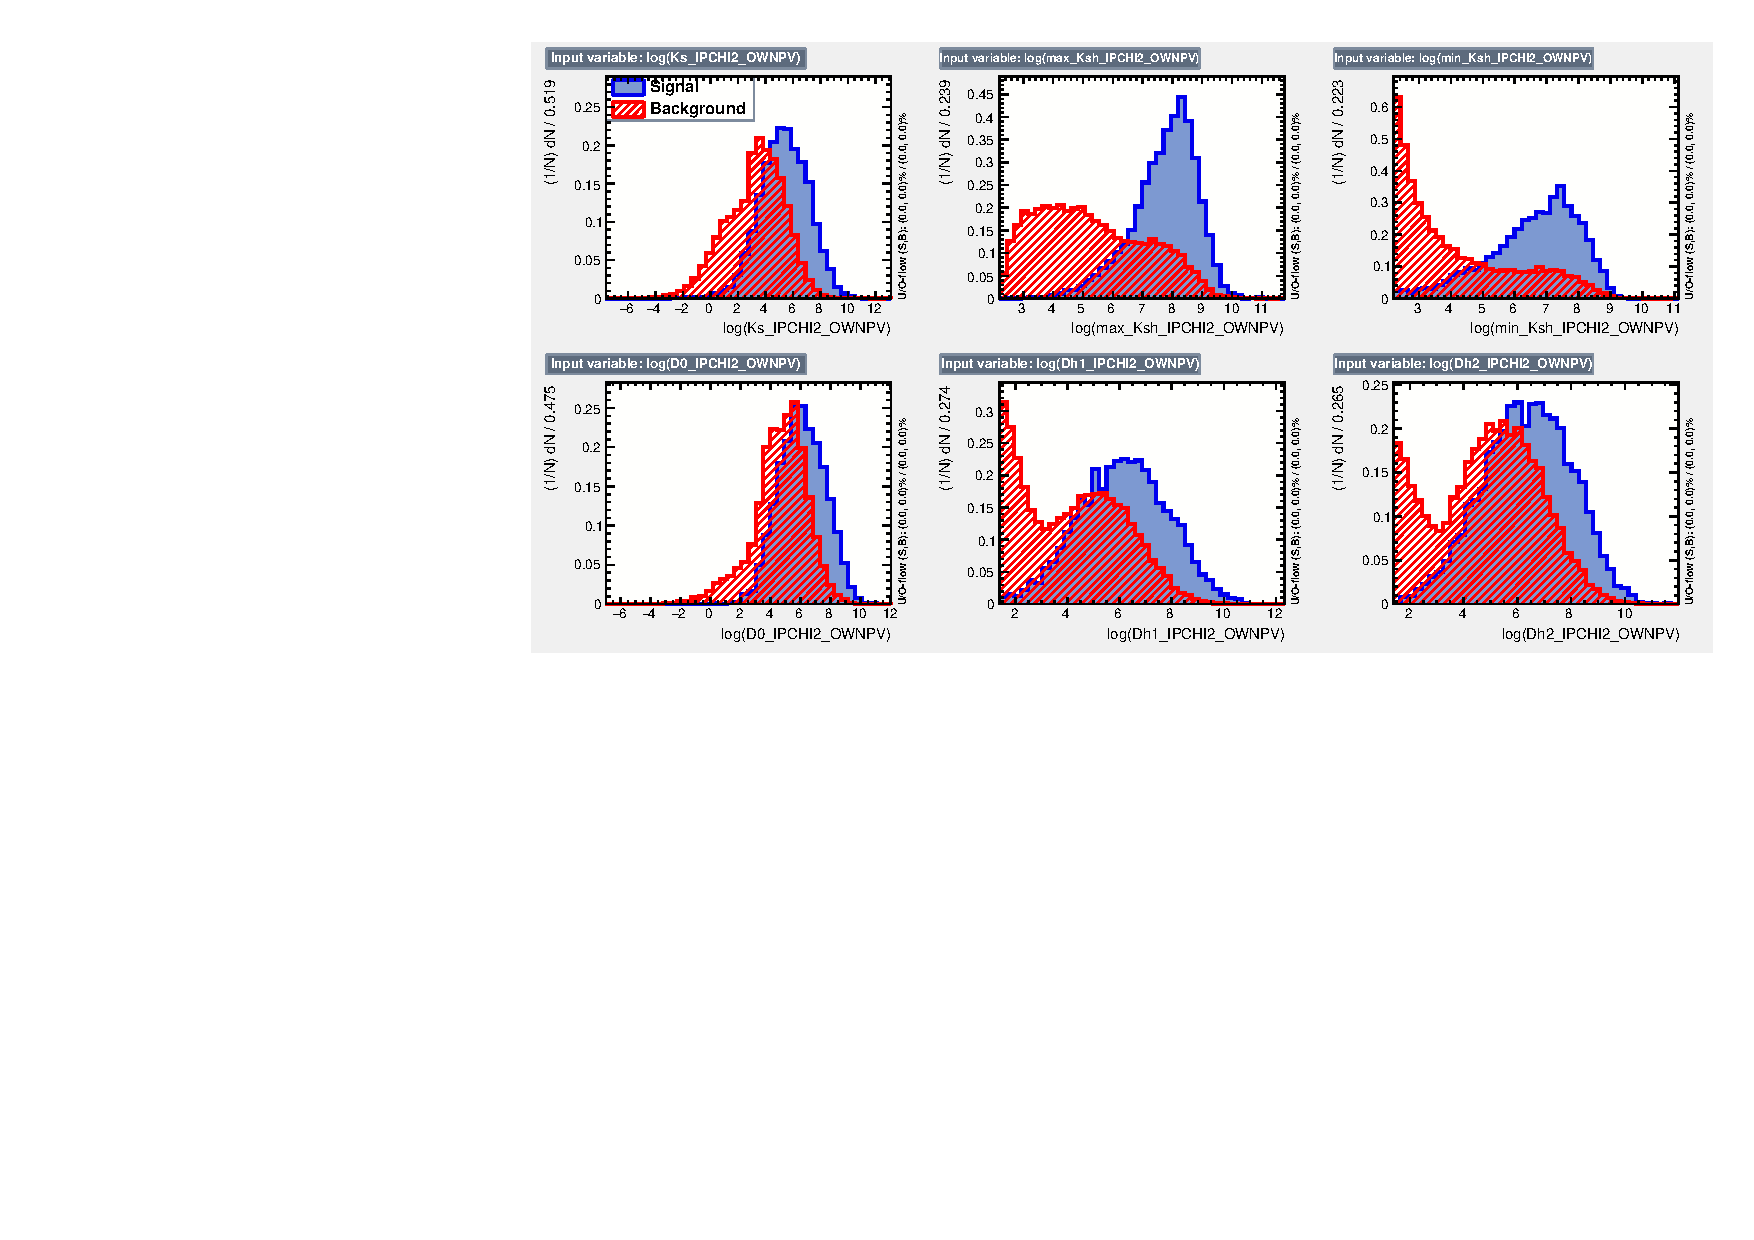
\includegraphics[width=\linewidth]{figures/selection/inputvariables_KPi_LL_run1_1.pdf}
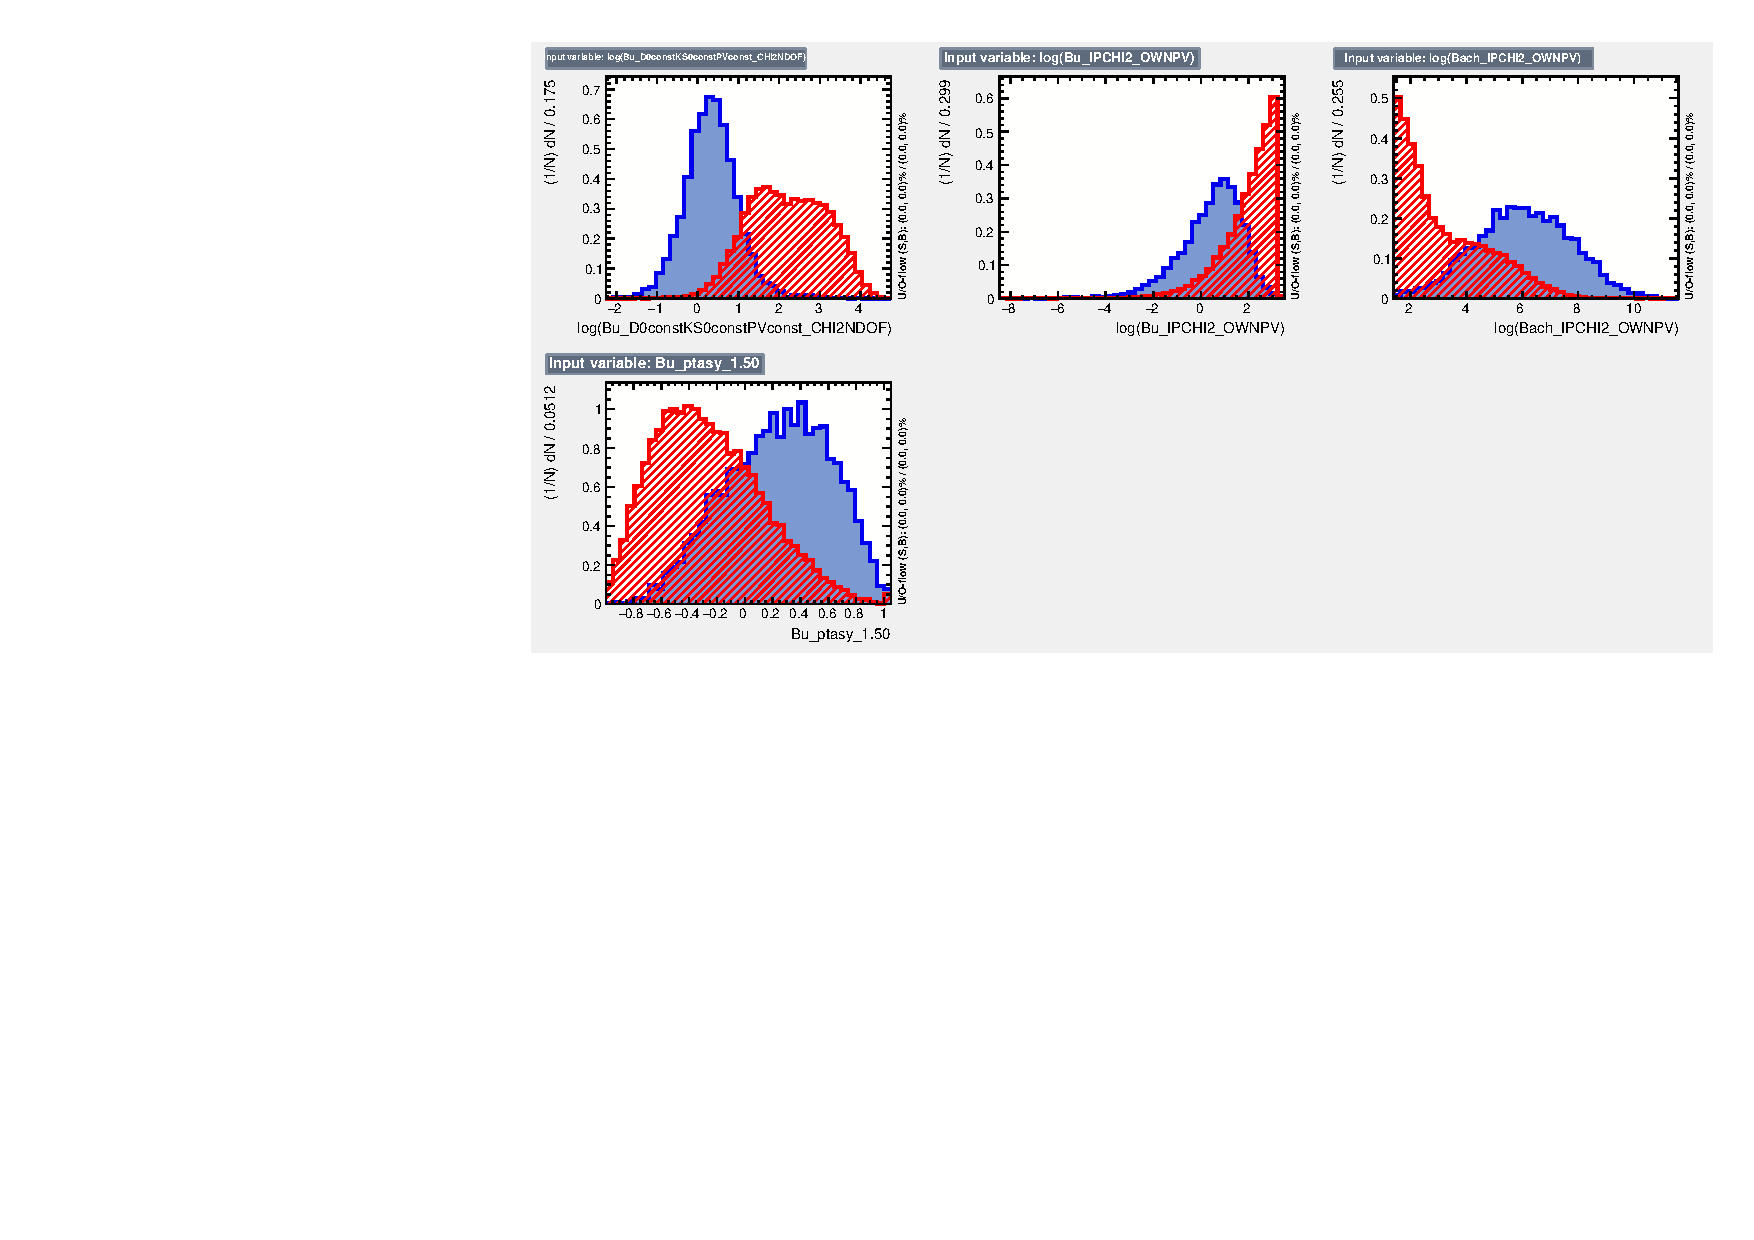
\includegraphics[width=\linewidth]{figures/selection/inputvariables_KPi_LL_run1_2.pdf}
\caption{BDT input variable distributions for signal and background for 2-body LL}
\label{BDTinputdist2bodyLL}
\end{figure}

\begin{figure}[tb]
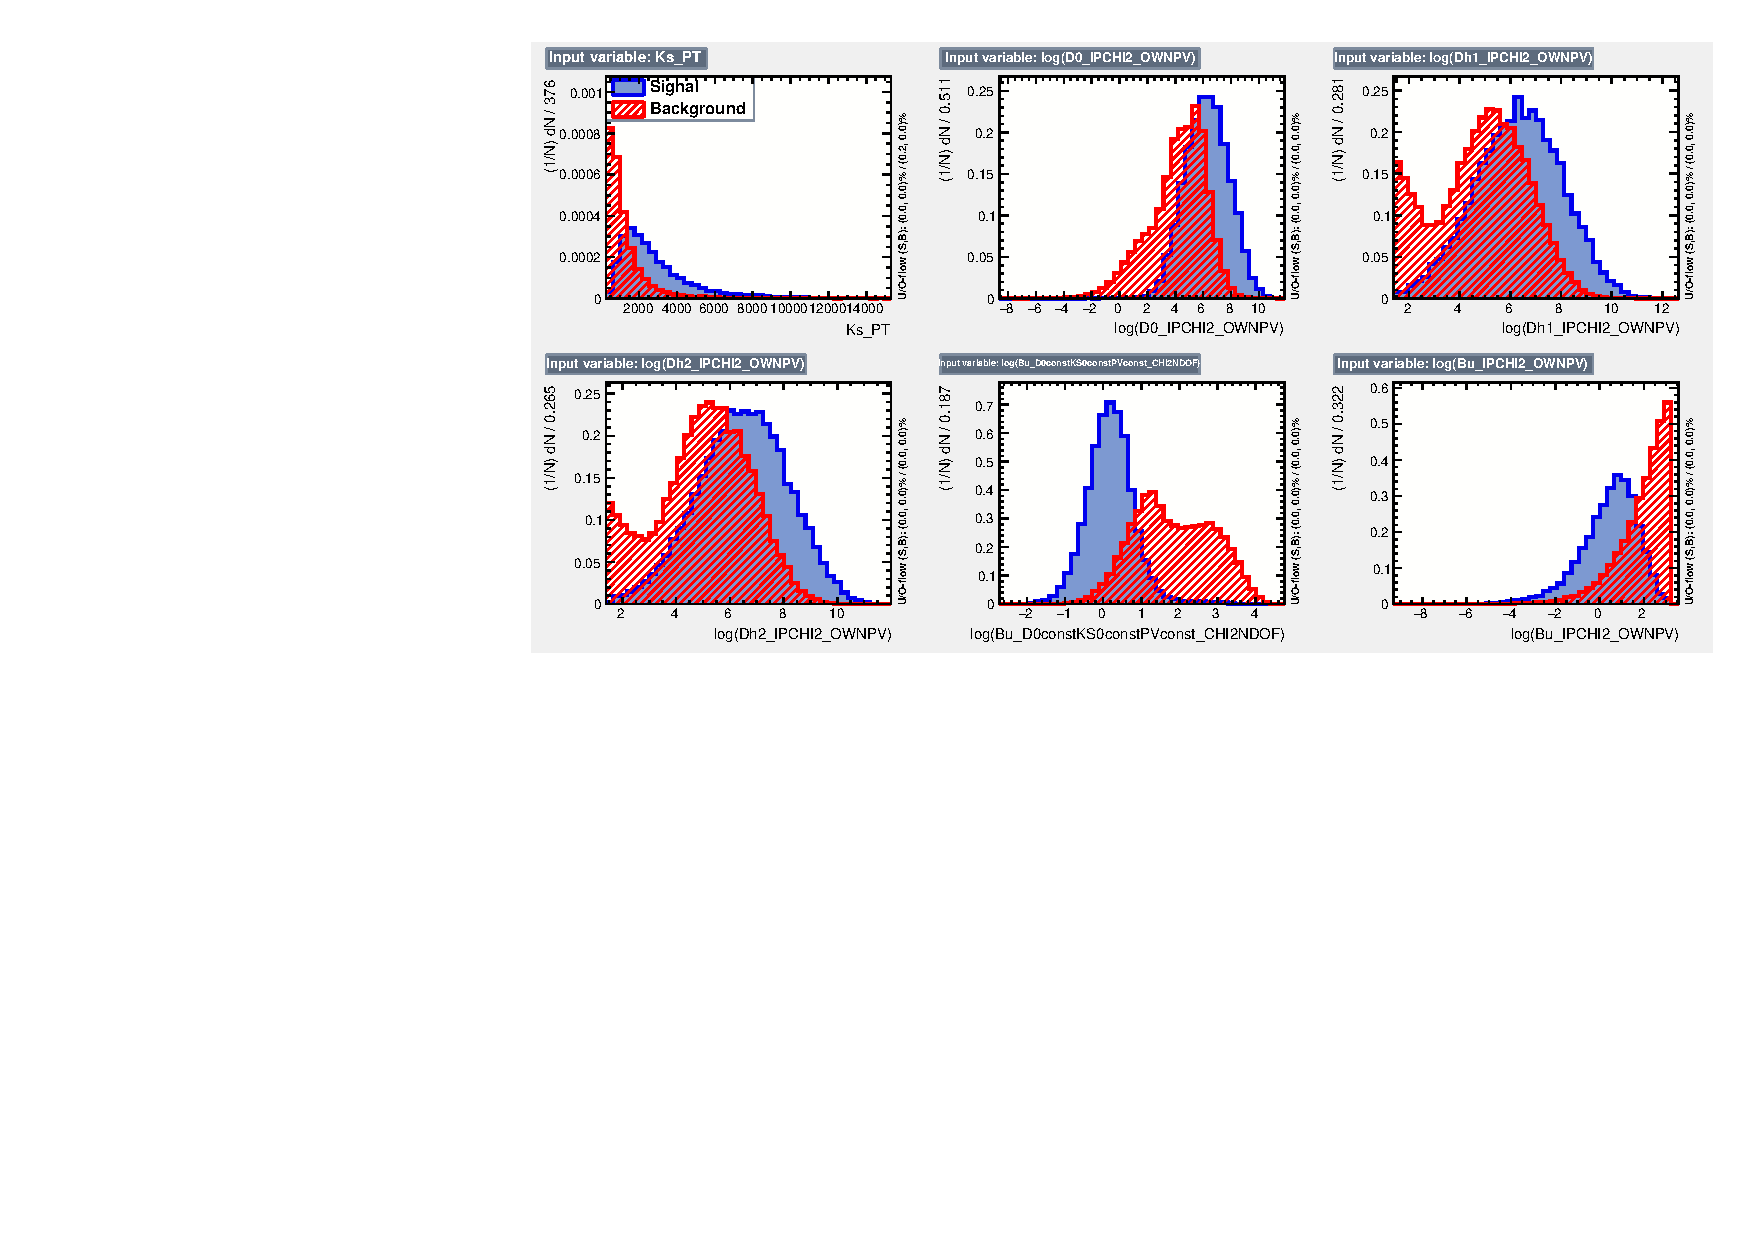
\includegraphics[width=\linewidth]{figures/selection/inputvariables_KPi_DD_run1_1.pdf}
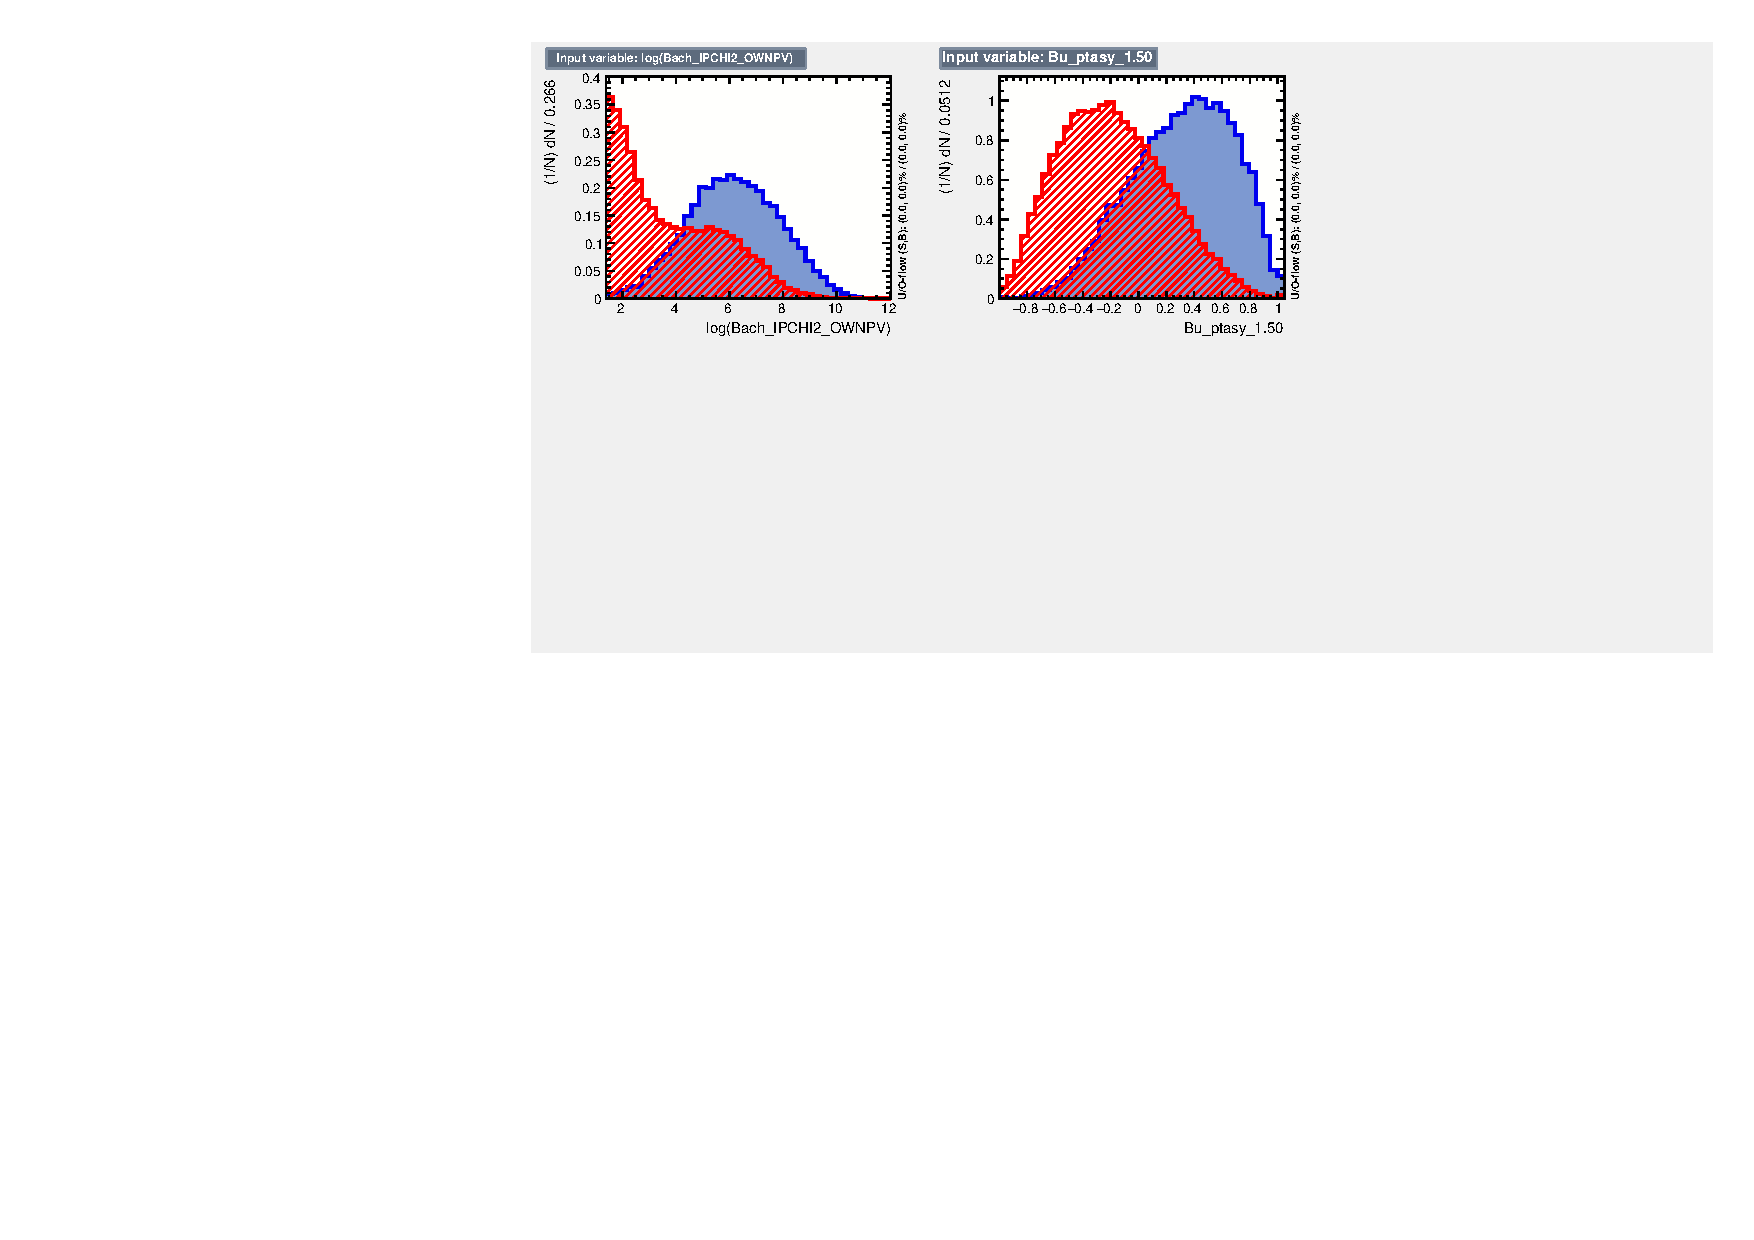
\includegraphics[width=\linewidth]{figures/selection/inputvariables_KPi_DD_run1_2.pdf}
\caption{BDT input variable distributions for signal and background for 2-body DD}
\label{BDTinputdist2bodyDD}
\end{figure}

\begin{figure}
\begin{verbatim}
BDTG_LL
-------------------------------------------------------------------------
Rank : Variable                                : Variable Importance
-------------------------------------------------------------------------
   1 : log(Bu_D0constKS0constPVconst_CHI2NDOF) : 1.396e-01
   2 : log(Ks_IPCHI2_OWNPV)                    : 1.266e-01
   3 : log(max_Ksh_IPCHI2_OWNPV)               : 1.024e-01
   4 : Bu_ptasy_1.50                           : 9.928e-02
   5 : log(Dh1_IPCHI2_OWNPV)                   : 9.739e-02
   6 : log(Bach_IPCHI2_OWNPV)                  : 9.650e-02
   7 : log(D0_IPCHI2_OWNPV)                    : 8.777e-02
   8 : log(min_Ksh_IPCHI2_OWNPV)               : 8.699e-02
   9 : log(Dh2_IPCHI2_OWNPV)                   : 8.290e-02
  10 : log(Bu_IPCHI2_OWNPV)                    : 8.056e-02
-------------------------------------------------------------------------

BDTG_DD
-------------------------------------------------------------------------
Rank : Variable                                : Variable Importance
-------------------------------------------------------------------------
   1 : log(Bu_D0constKS0constPVconst_CHI2NDOF) : 1.459e-01
   2 : log(Dh1_IPCHI2_OWNPV)                   : 1.287e-01
   3 : log(Bach_IPCHI2_OWNPV)                  : 1.280e-01
   4 : Bu_ptasy_1.50                           : 1.260e-01
   5 : log(Dh2_IPCHI2_OWNPV)                   : 1.214e-01
   6 : log(D0_IPCHI2_OWNPV)                    : 1.174e-01
   7 : log(Bu_IPCHI2_OWNPV)                    : 1.171e-01
   8 : Ks_PT                                   : 1.155e-01
-------------------------------------------------------------------------
\end{verbatim}
\caption{Ranking for variables for BDTG\_LL and BDTG\_DD for the two body BDTs}
\label{variableranking2body}
\end{figure}

\begin{figure}[tb]
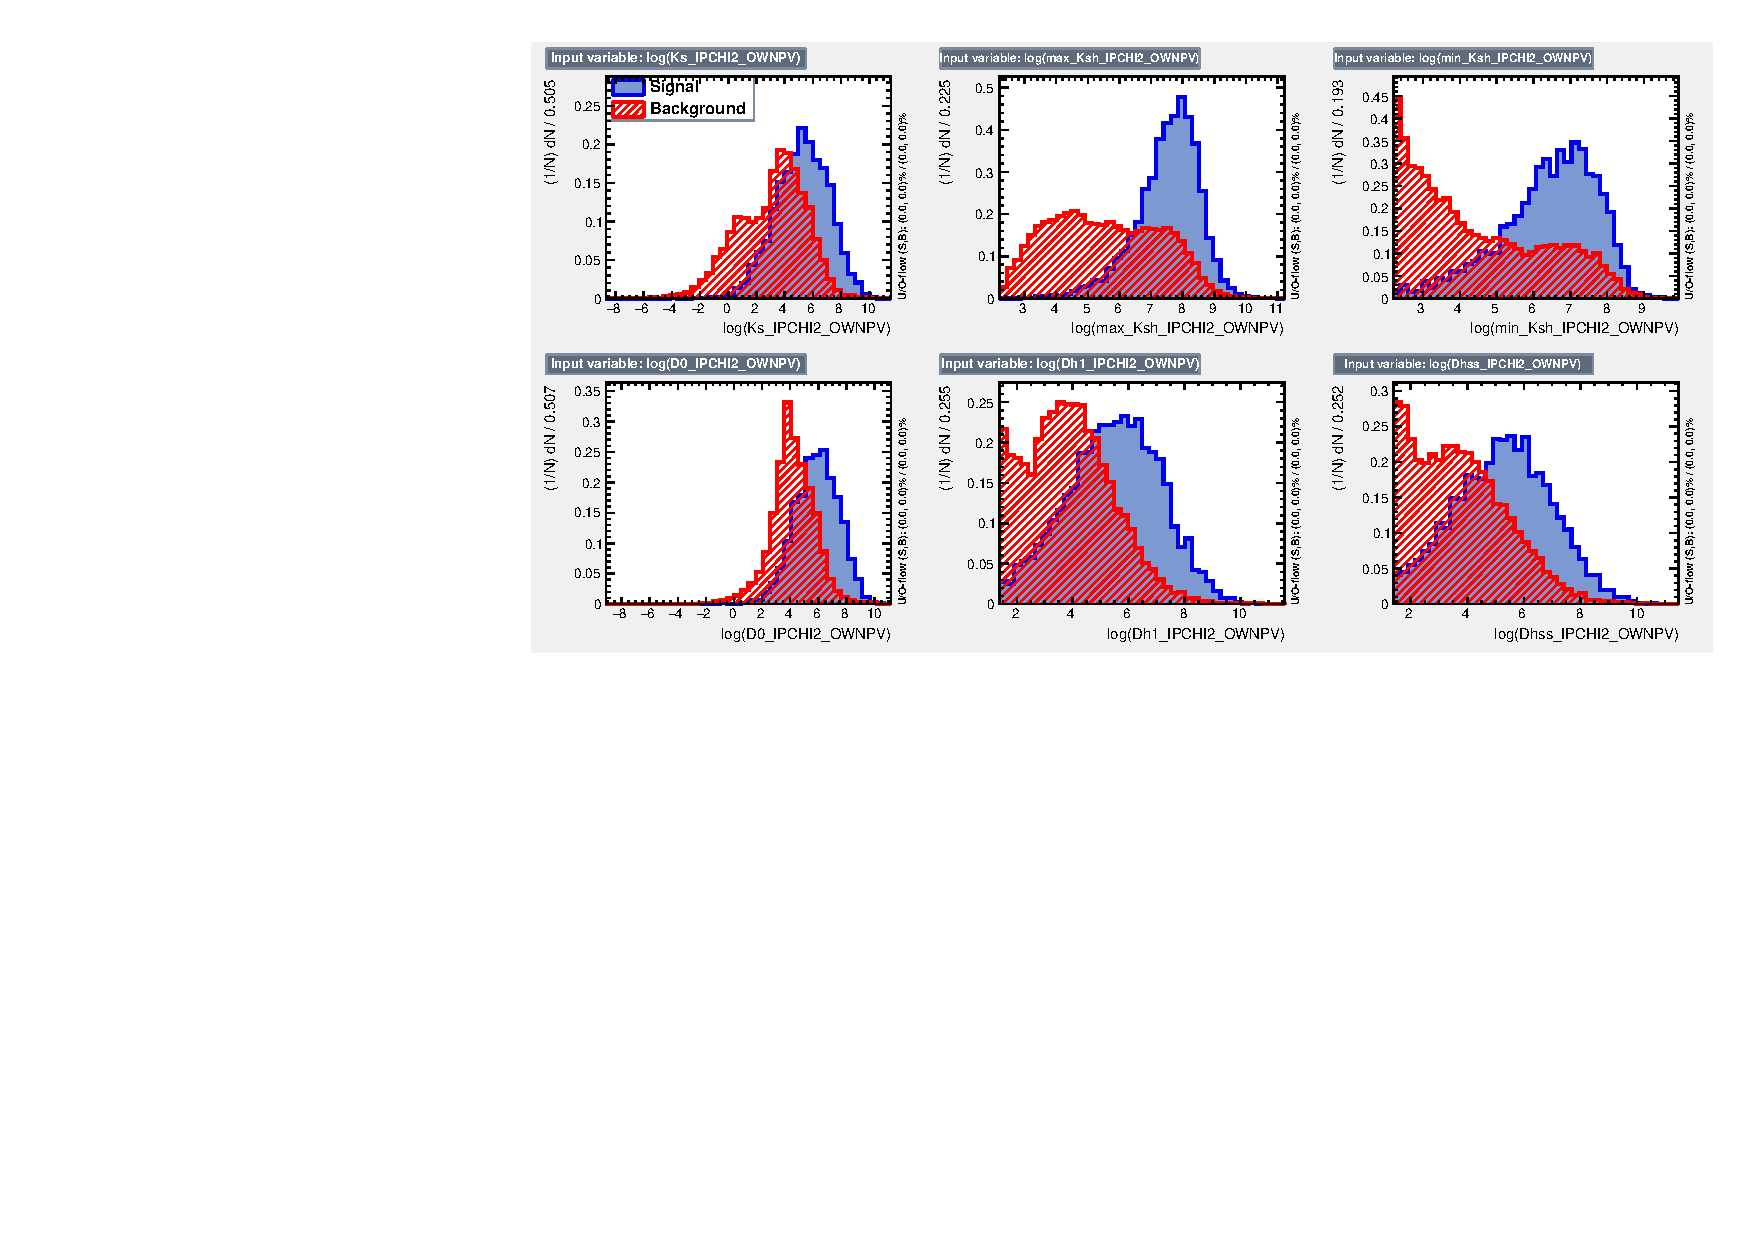
\includegraphics[width=\linewidth]{figures/selection/inputvariables_KPiPiPi_LL_run2_1.pdf}
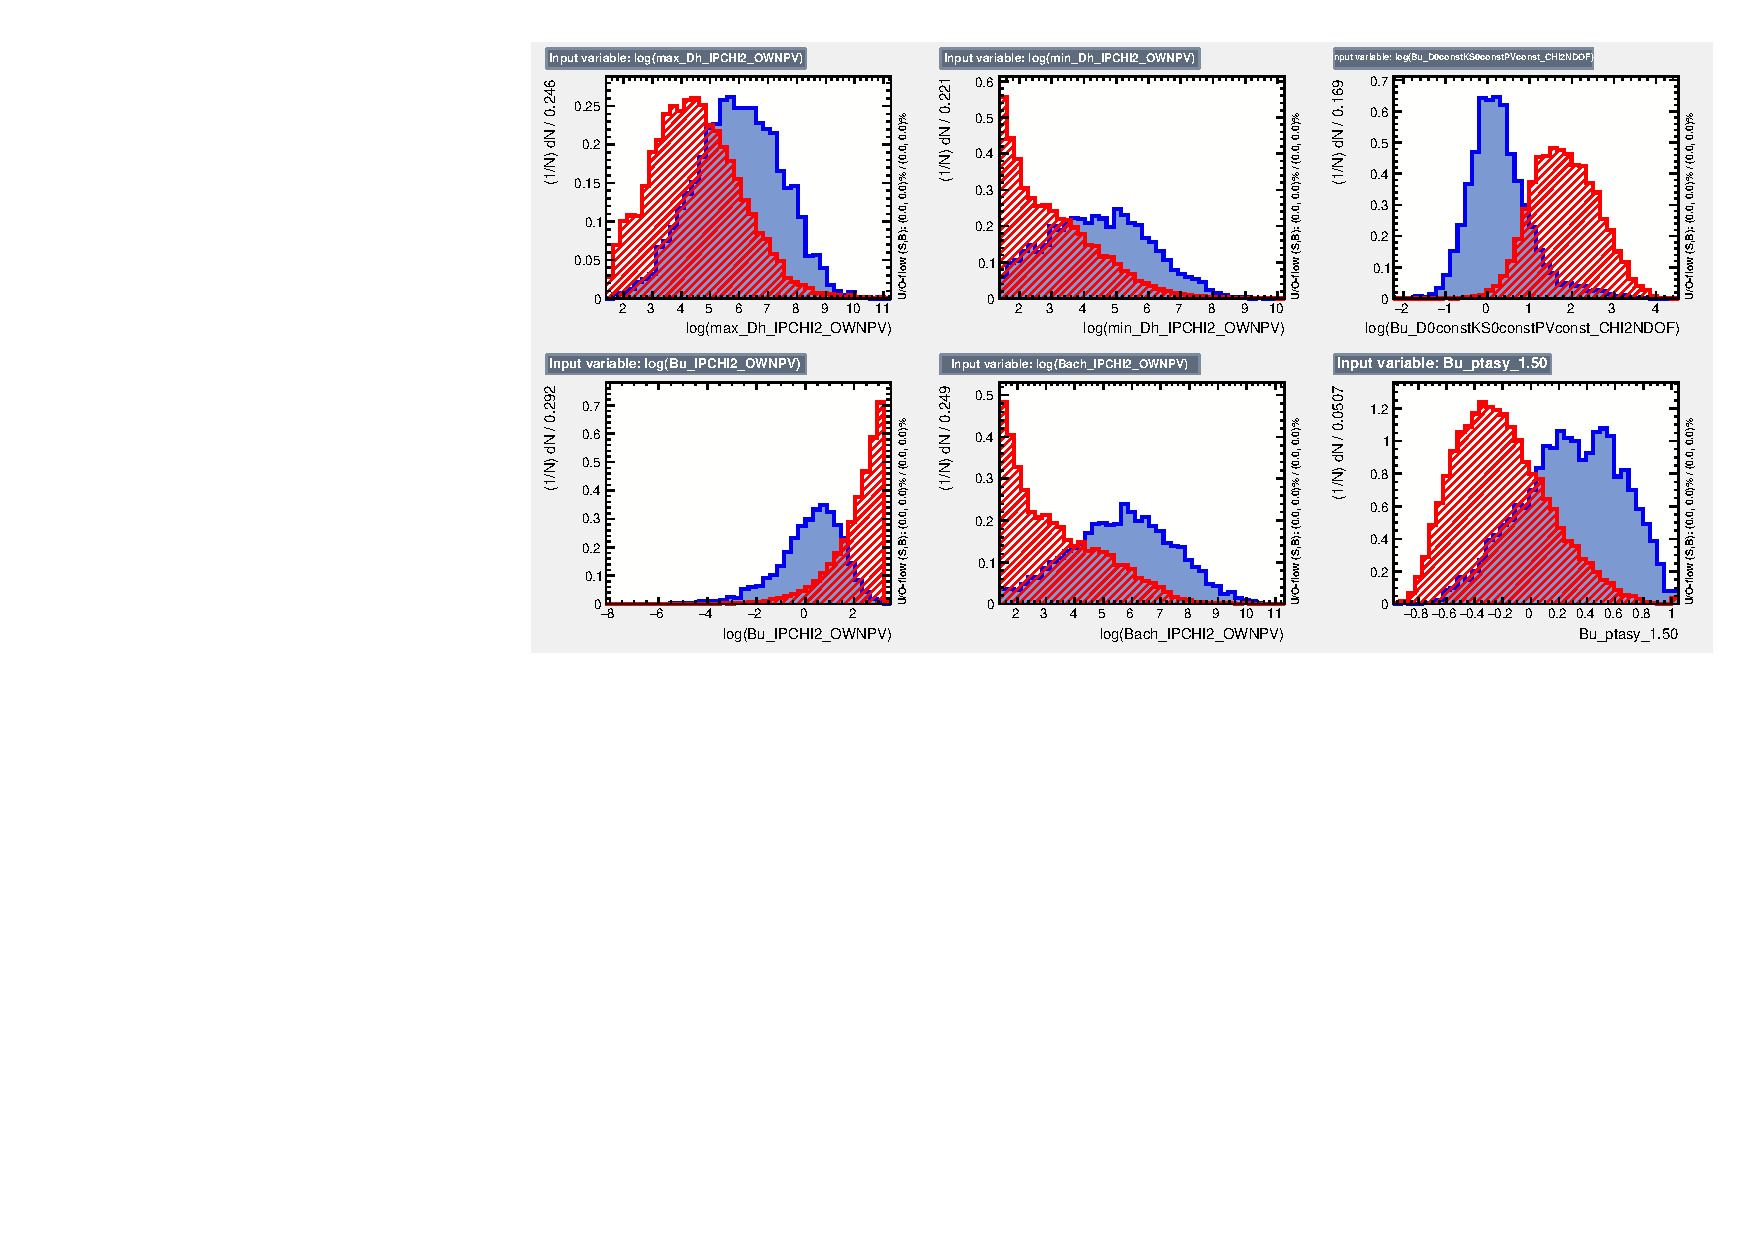
\includegraphics[width=\linewidth]{figures/selection/inputvariables_KPiPiPi_LL_run2_2.pdf}
\caption{BDT input variable distributions for signal and background for 4-body LL}
\label{BDTinputdist4bodyLL}
\end{figure}

\begin{figure}[tb]
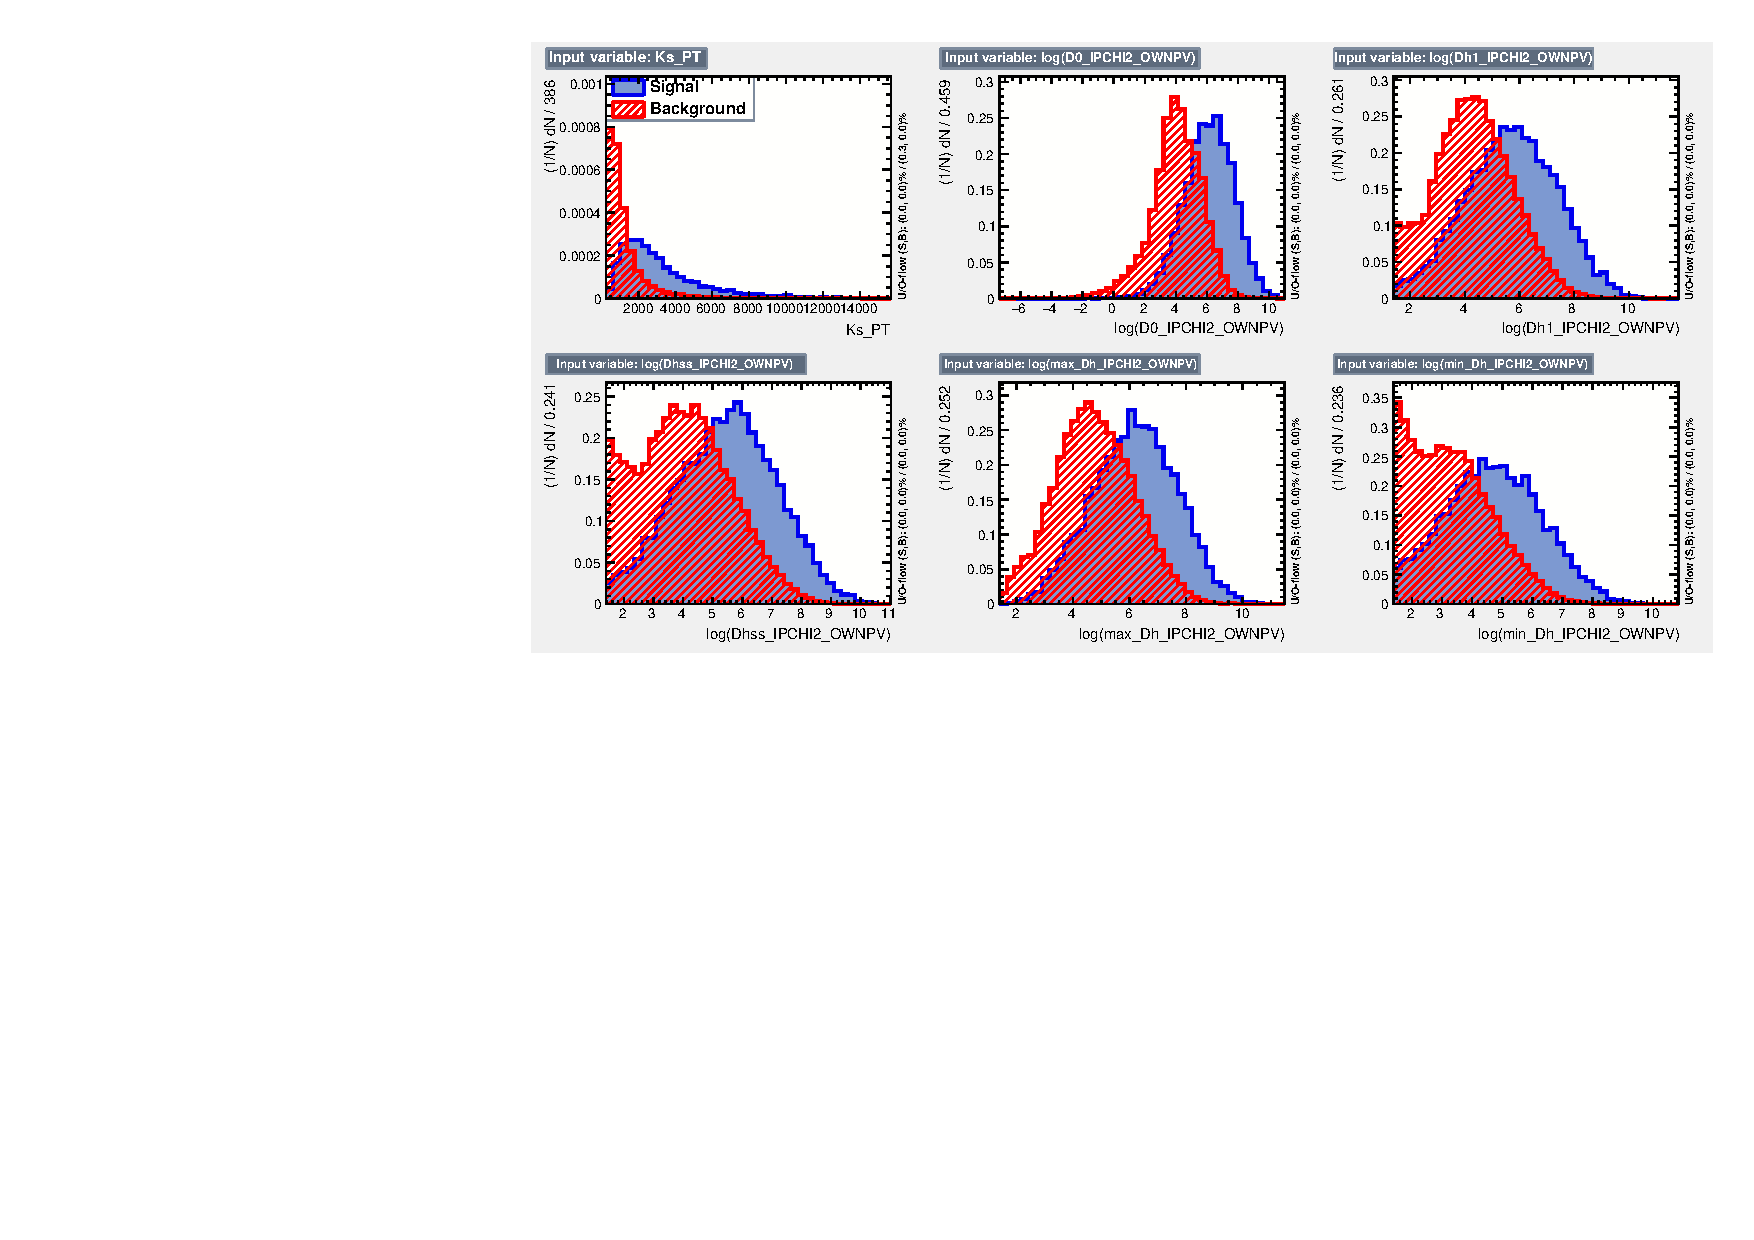
\includegraphics[width=\linewidth]{figures/selection/inputvariables_KPiPiPi_DD_run2_1.pdf}
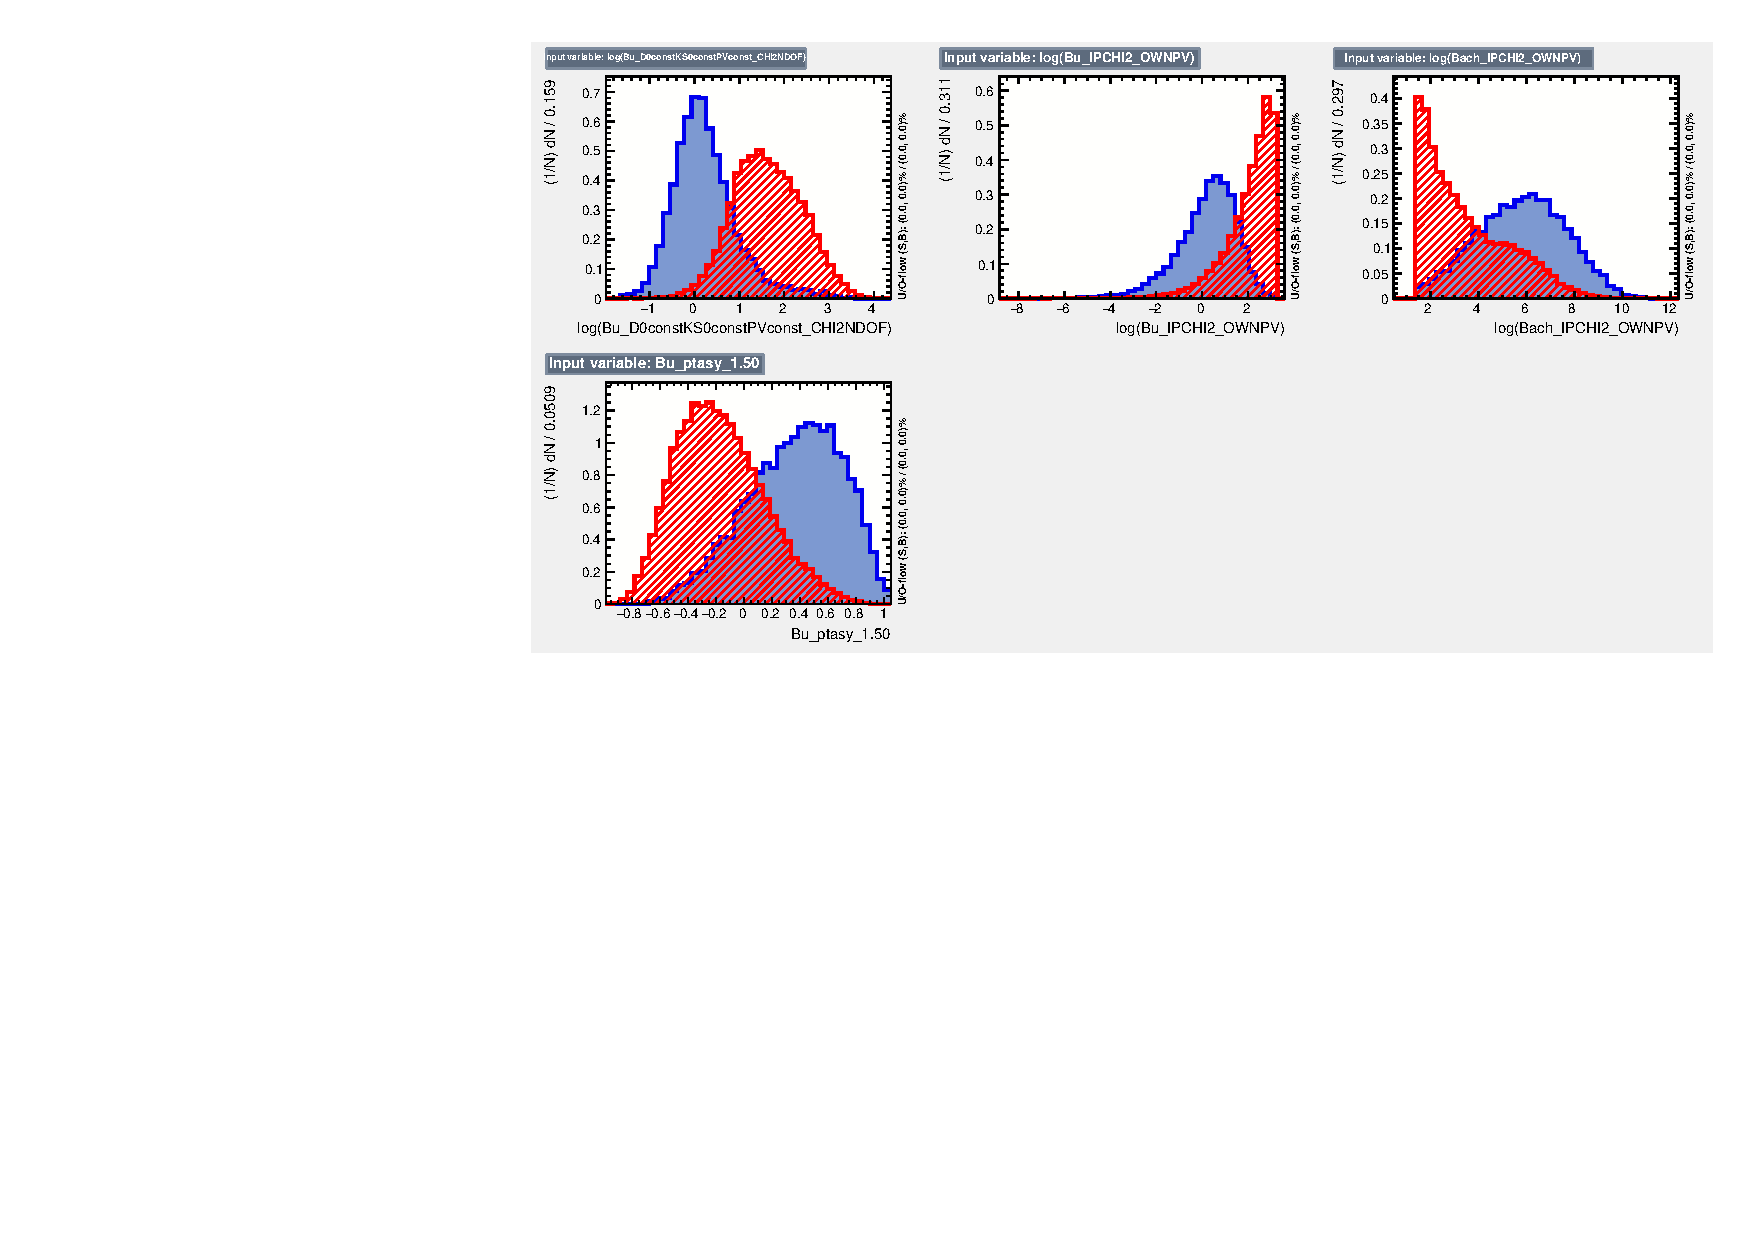
\includegraphics[width=\linewidth]{figures/selection/inputvariables_KPiPiPi_DD_run2_2.pdf}
\caption{BDT input variable distributions for signal and background for 4-body DD}
\label{BDTinputdist4bodyDD}
\end{figure}

\begin{figure}
\begin{verbatim}
BDTG_LL
-------------------------------------------------------------------------
Rank : Variable                                : Variable Importance
-------------------------------------------------------------------------
   1 : log(Bu_D0constKS0constPVconst_CHI2NDOF) : 1.109e-01
   2 : log(Ks_IPCHI2_OWNPV)                    : 1.028e-01
   3 : Bu_ptasy_1.50                           : 9.283e-02
   4 : log(Bu_IPCHI2_OWNPV)                    : 8.911e-02
   5 : log(D0_IPCHI2_OWNPV)                    : 8.245e-02
   6 : log(Dh1_IPCHI2_OWNPV)                   : 7.997e-02
   7 : log(Bach_IPCHI2_OWNPV)                  : 7.899e-02
   8 : log(min_Dh_IPCHI2_OWNPV)                : 7.513e-02
   9 : log(max_Ksh_IPCHI2_OWNPV)               : 7.480e-02
  10 : log(Dhss_IPCHI2_OWNPV)                  : 7.469e-02
  11 : log(min_Ksh_IPCHI2_OWNPV)               : 7.295e-02
  12 : log(max_Dh_IPCHI2_OWNPV)                : 6.546e-02
-------------------------------------------------------------------------

BDTG_DD
-------------------------------------------------------------------------
Rank : Variable                                : Variable Importance
-------------------------------------------------------------------------
   1 : log(Bu_D0constKS0constPVconst_CHI2NDOF) : 1.251e-01
   2 : Bu_ptasy_1.50                           : 1.108e-01
   3 : log(Bu_IPCHI2_OWNPV)                    : 1.080e-01
   4 : log(Bach_IPCHI2_OWNPV)                  : 1.056e-01
   5 : Ks_PT                                   : 1.054e-01
   6 : log(D0_IPCHI2_OWNPV)                    : 1.052e-01
   7 : log(max_Dh_IPCHI2_OWNPV)                : 9.205e-02
   8 : log(Dhss_IPCHI2_OWNPV)                  : 8.864e-02
   9 : log(Dh1_IPCHI2_OWNPV)                   : 8.393e-02
  10 : log(min_Dh_IPCHI2_OWNPV)                : 7.533e-02
-------------------------------------------------------------------------
\end{verbatim}
\caption{Ranking for variables for BDTG\_LL and BDTG\_DD for the four body BDTs}
\label{variableranking4body}
\end{figure}

\begin{figure}[tb]
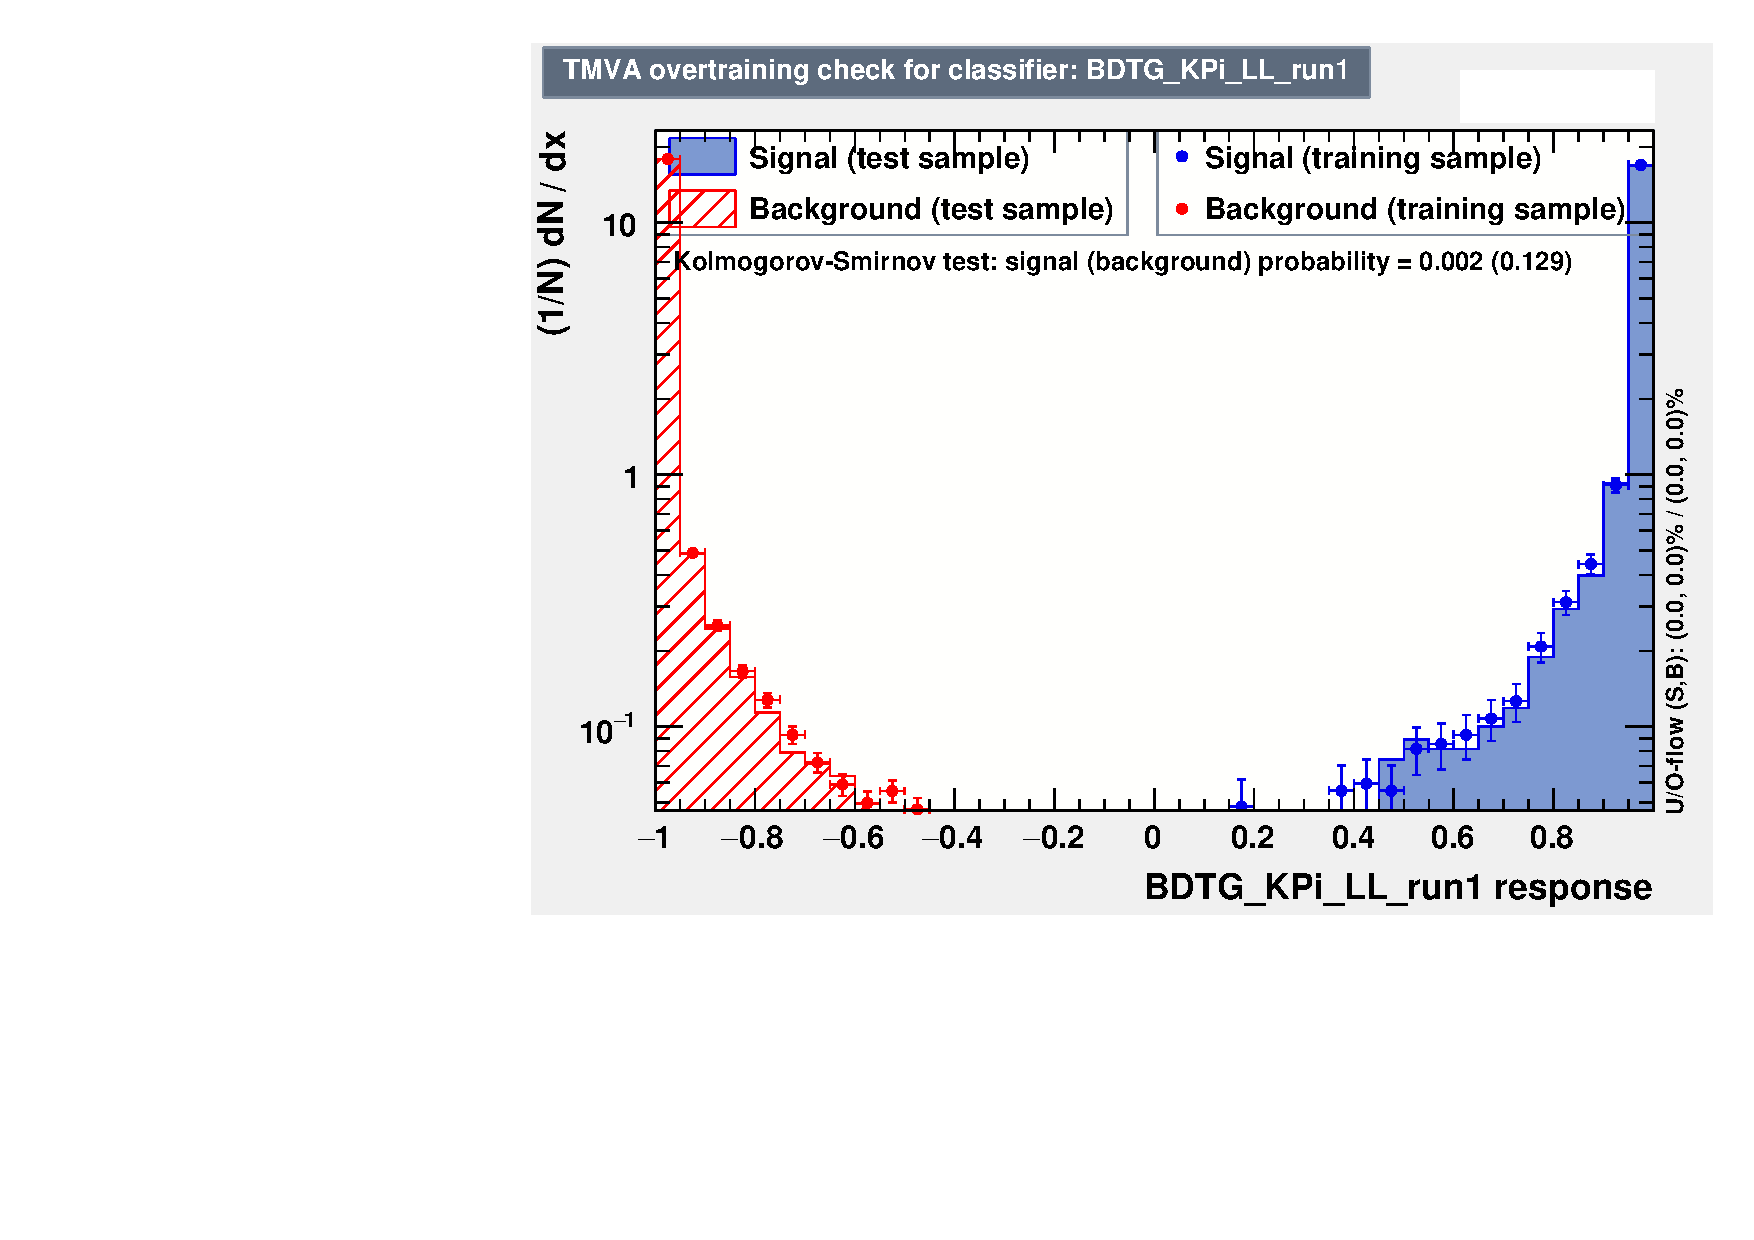
\includegraphics[width=0.5\linewidth]{figures/selection/overtraining_KPi_LL_run1.pdf}
\put(-150,100) {(a)}
\hfill
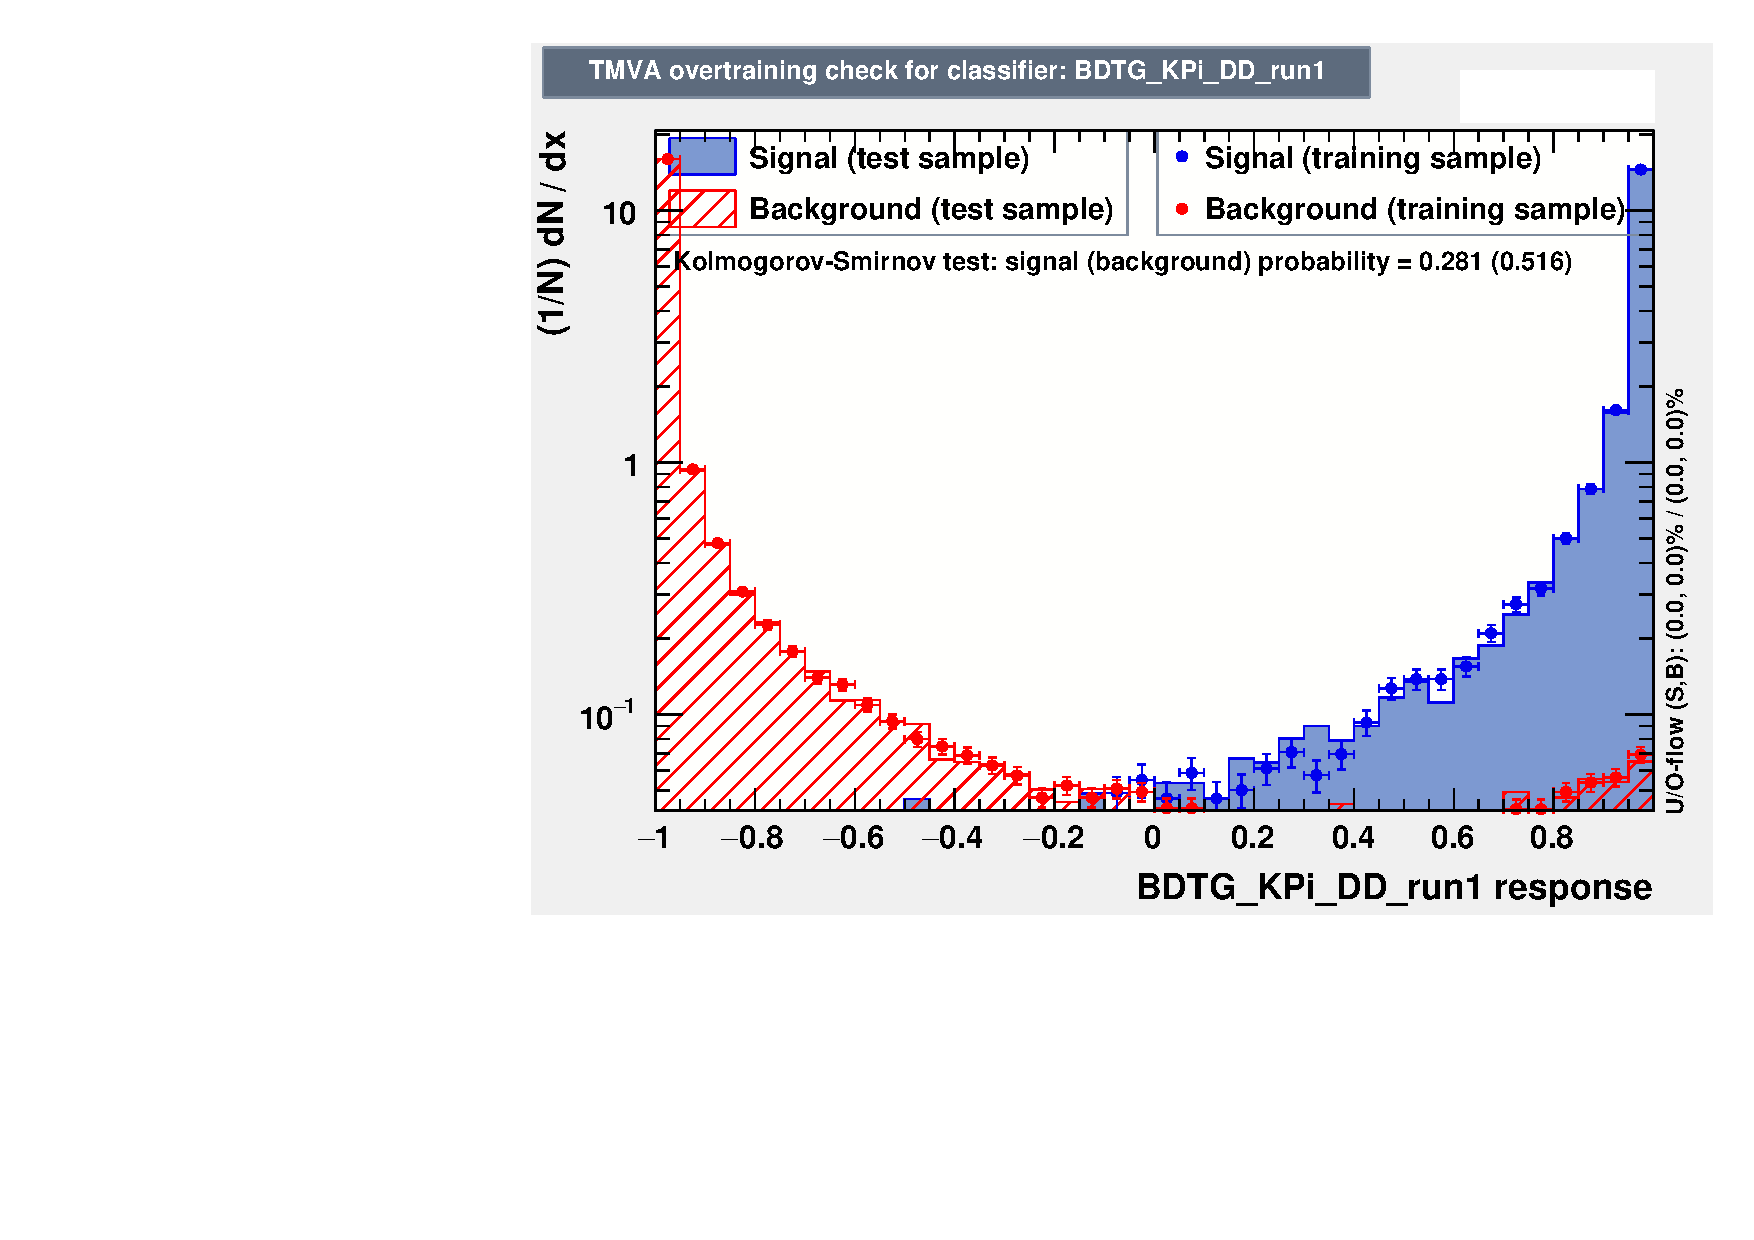
\includegraphics[width=0.5\linewidth]{figures/selection/overtraining_KPi_DD_run1.pdf}
\put(-140,100) {(b)}
\hfill
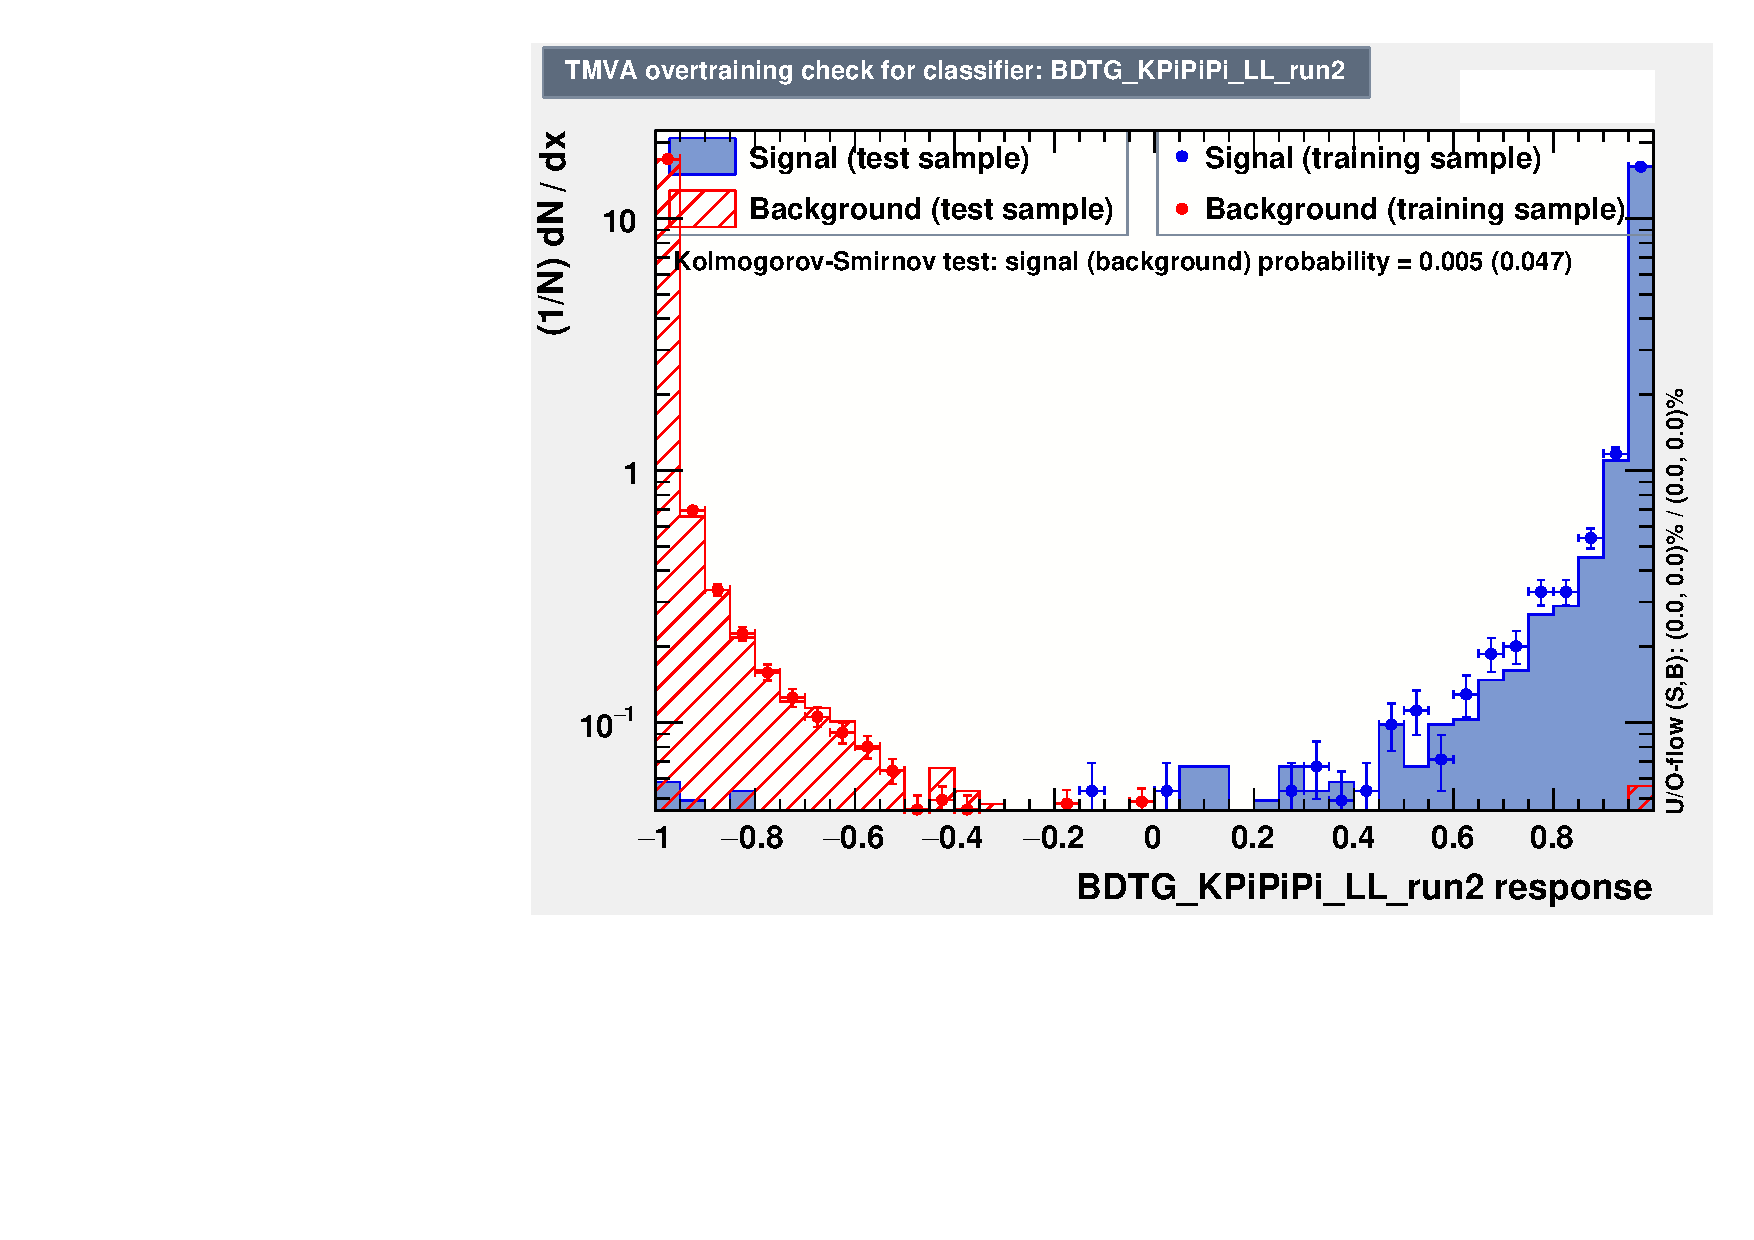
\includegraphics[width=0.5\linewidth]{figures/selection/overtraining_KPiPiPi_LL_run2.pdf}
\put(-150,100) {(c)}
\hfill
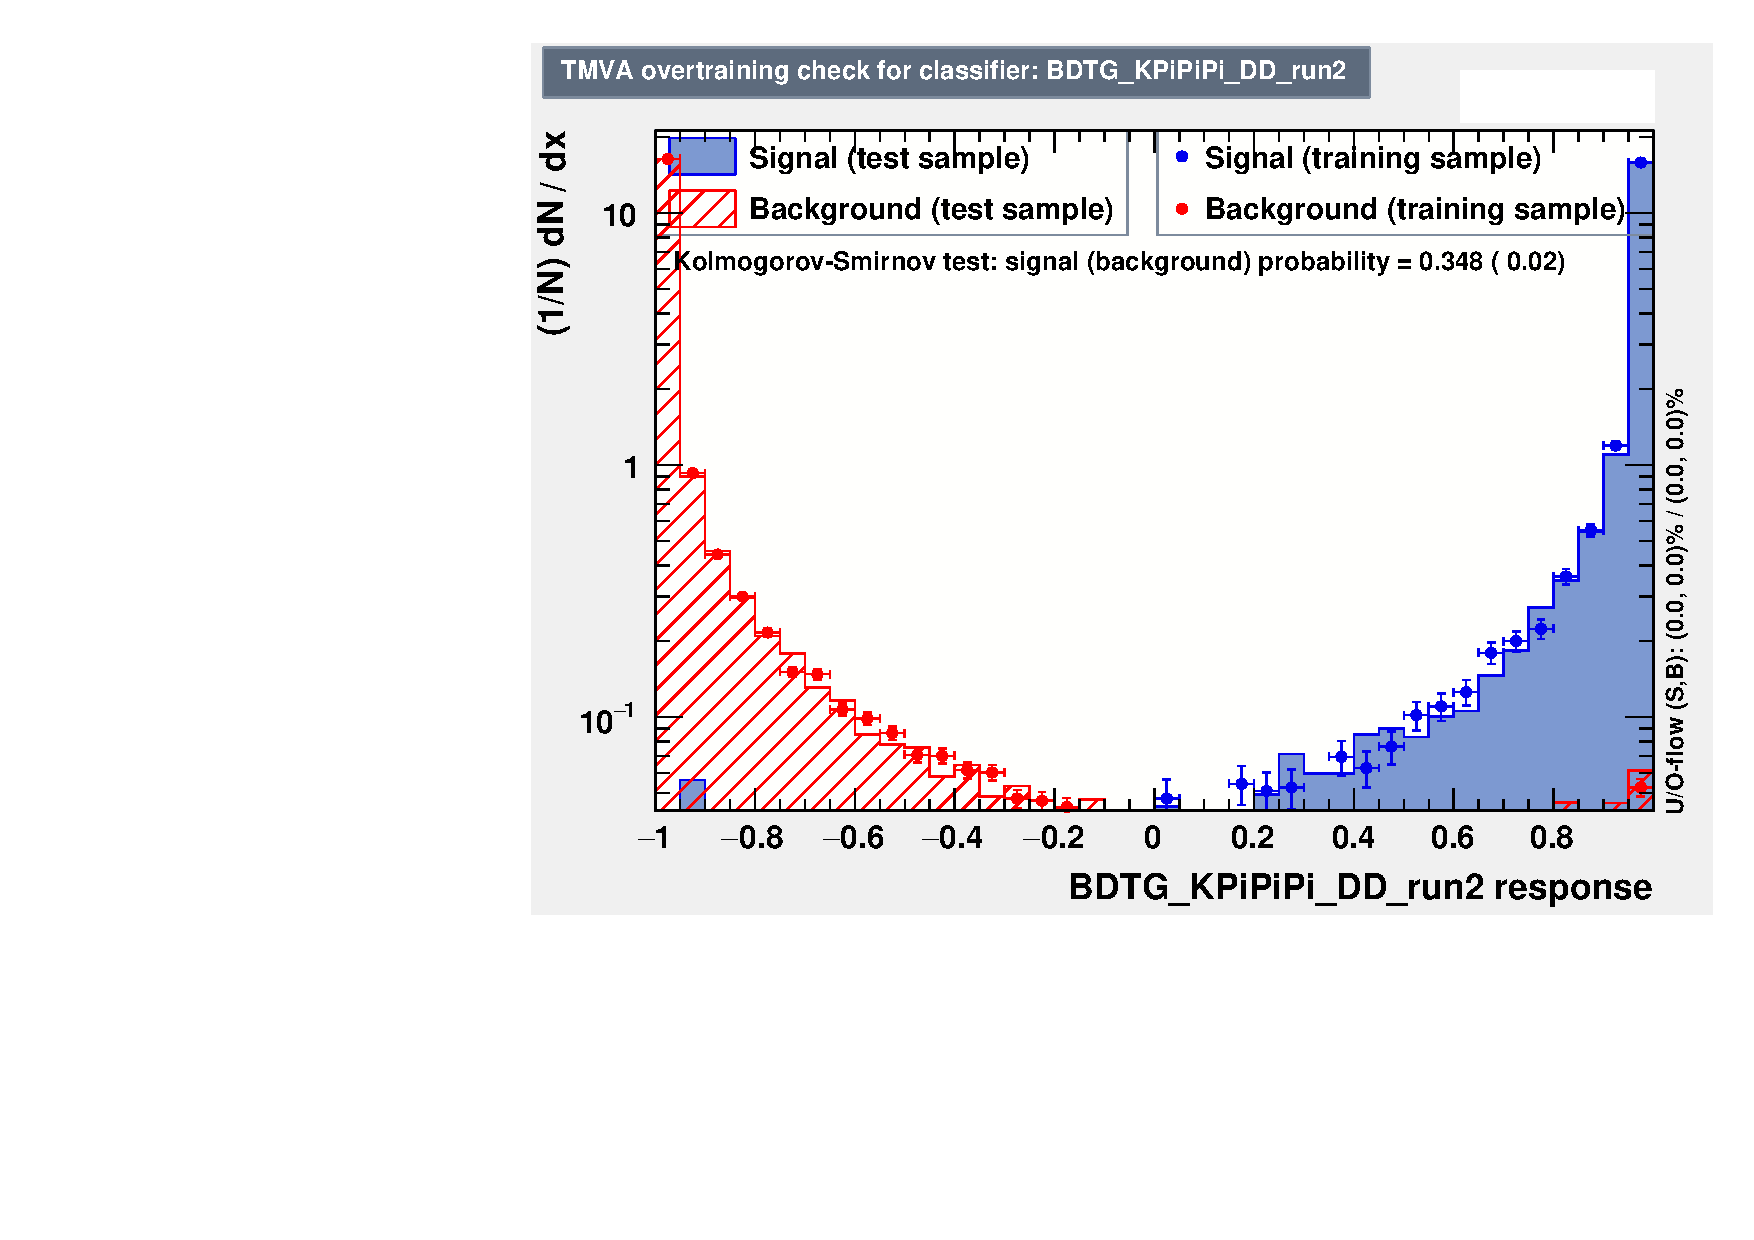
\includegraphics[width=0.5\linewidth]{figures/selection/overtraining_KPiPiPi_DD_run2.pdf}
\put(-140,100) {(d)}
\caption{Training and test distributions from TMVA for (a) 2-body BDT\_LL, (b) 2-body BDT\_DD, (c) 4-body BDT\_LL and (d) 4-body BDT\_DD}
\label{BDTovertraining}
\end{figure}

Other selection strategies were explored. Multiple BDTs were investigated, by training and implementing a \KS BDT and a \Dz BDT followed by a B BDT. Two approaches were tried: one using the same set of variables in all three BDTs and one using variables relating to the \KS in the \KS BDT and variables relating to the \Dz in the \Dz BDT. These methods were found to have little or no improvement on the single BDT. Many other variables were investigated in the BDT, including kinematic variables of the B and D. These were found to give no significant improvement in BDT performance. A 2-body BDT trained on Run 2 data and MC was investigated to apply to Run 2 data, which did not result in any improvement in performance compared to the BDT trained on Run 1. Therefore, it was not considered necessary to have BDTs trained separately for Run 1 and Run 2.

For the 2-body BDTs, a BDT selection of 0.6 is chosen for BDT\_LL and 0.7 for BDT\_DD for all D modes except the ADS mode. The ADS mode BDT selection is chosen to be 0.6 for BDT\_LL and 0.9 for BDT\_DD. This tighter BDT selection is justified in Figure \ref{adsoptimisation}. When applied to the $K\pi$ favoured mode in Run 1 the BDT selection gives a 95\% signal efficiency and 96\% background rejection for LL and 88\% signal efficiency and 94\% background rejection for DD. The signal efficiencies of the BDT cuts are given in Table \ref{bdtefficiencies2body}. These BDT selections, in conjuction with the \Kstarm mass window and \KS helicity angle, were optimised to reduce the fit error on the physics observables, as detailed in Section \ref{sec:cpfit:optimisation}. Many toy studies were run to calculate the fit uncertainty for each selection. To optimise the selection for the GLW modes, the fit error was minimised for $A_{KK}$, $R_{KK}$, $A_{\pi\pi}$ and $R_{\pi\pi}$. The BDT selection for the ADS modes was optimised to minimise the fit errors in $R^+$ and $R^-$, as illustated in Figure \ref{adsoptimisation}. 

In cases when the figure of merits in these optimisation studies were not especially sensitive to changes in the selection, the selection giving the highest coherence (i.e most stringent requirement on the \Kstarm) was chosen and the BDT signal and background efficiencies were taken into account.

For the four-body modes the same optimisation point was chosen 0.6 for BDT\_LL and 0.7 for BDT\_DD for the \decay{\Dz}{\Kp\pim\pip\pim} \decay{\Dz}{\pi\pi\pi\pi} mode, and 0.6 for BDT\_LL and 0.9 for BDT\_DD for the \decay{\Dz}{\Kp\pim\pip\pim} mode. The optimisation point was verified by minimising the fit error in toys for $A_{K\pi\pi\pi}$, $R^+_{K\pi\pi\pi}$ and $R^-_{K\pi\pi\pi}$.


\subsection{Other cuts}

Some other selection requirements are implemented to tackle certain backgrounds.

\begin{itemize}
\item{\textbar $\cos$(Ks helicity angle) \textbar $>$ 0.3, discussed in Section \ref{sec:backgrounds:non-resonant}. This angle is defined as is the angle between the \KS and the bachelor pion in the \Kstarm rest frame}
\item{\Dz FD significance $>$ 2 is required to remove charmless backgrounds, discussed in Section \ref{sec:backgrounds:charmless}}
\item{\KS FD significance $>$ 5 (for LL candidates only) is required to remove $B \to D\pi\pi\pi$ background, discussed in Section \ref{sec:backgrounds:b2dpipipi}}
\item{15 MeV double misID veto, discussed further in Section \ref{sec:backgrounds:crossfeed}}
\begin{itemize}
\item For two-body: 15 MeV double misID veto is applied to $B^{\pm} \to [K^{\mp}\pi^{\pm}] K^{*\pm}$ only. The \Dz mass is reconstructed where both daughter mass hypotheses are swapped (kaon reconstructed as a pion and pion reconstructed as a kaon), this is required to be greater than 15 MeV away from the nominal \Dz mass.
\item For four-body: There are two possible pions that could be incorrectly reconstructed as a kaon, therefore two 15 MeV double misID vetos are applied to both the favoured and the supressed modes. 
\end{itemize} 
\end{itemize}


\subsection{PID selection}
\label{sec:selection:pid}

The selection requirements are identical for each of the different D modes, $K\pi$, $KK$, $\pi\pi$ and $\pi K$, with the exception of the double misID veto. Therefore, it is essential to apply PID selection that efficiently distinguishes between pions and kaons. The PID cuts on the daughters of the D meson are designed so that no \decay{\Dz}{hh} candidate can appear in more than one category with a change in mass hypothesis. A PID requirement must be made on the bachelor pion in order to remove the \decay{\B}{\D\KS\kaon} background; this is discussed in more detail in Section \ref{sec:backgrounds:b2dkks}. 

For the bachelor PID (pion coming from the \Kstarm) a requirement of PIDK $<$ 4 is applied. For the 2-body D modes the requirements on the D daughters are kaons must satisfy DLLK $>$ 2 and pions must satifsfy DLLK $<$ -2. For the \decay{\Dz}{K\pi\pi\pi} modes, e.g. \decay{\Dz}{\Km\pip\pim\pip}, the \Km must satisfy DLLK $>$ 2 and both \pip must satifsfy DLLK $<$ -2; no PID requirement is applied for the \pip. For the \decay{\Dz}{\pip\pim\pip\pim}, the two \pip mesons must satisfy DLLK $<$ -2 and no PID requirements is placed on the \pim mesons. The PID requirements are the same as those used in the \decay{\Bp}{\D\Kp} analysis~\cite{LHCB-PAPER-2016-003}. No PID requirements are made on the \KS daughters; the high purity of the \KS means that this is not necessary, this is justified in Section \ref{sec:backgrounds:contamination}. The efficiency of this PID selection for the $K\pi$ favoured mode in Run 1 is 74\% and the efficiency of $\pi K$ events in the favoured mode is 0.15\%. These efficiencies are discussed in more detail in Section \ref{sec:mc:pid}. 


A brief look at ProbNN variables was undertaken early on in the analysis but cuts were not found that improved on the DLL cuts. Figure \ref{pidoptimisation} shows the variation of PID efficiencies with different selections. These results are based on a preliminary version of the selection and so the DLLK efficiencies are not the same as those quoted in this analysis.  The same PID selection is applied to both Run 1 and Run 2 datasets. It was found that for the given PID selection both PID efficiency and misID efficiency were improved for Run 2 compared to Run 1. More detail is given in Section \ref{sec:mc:pid}.

\begin{figure}
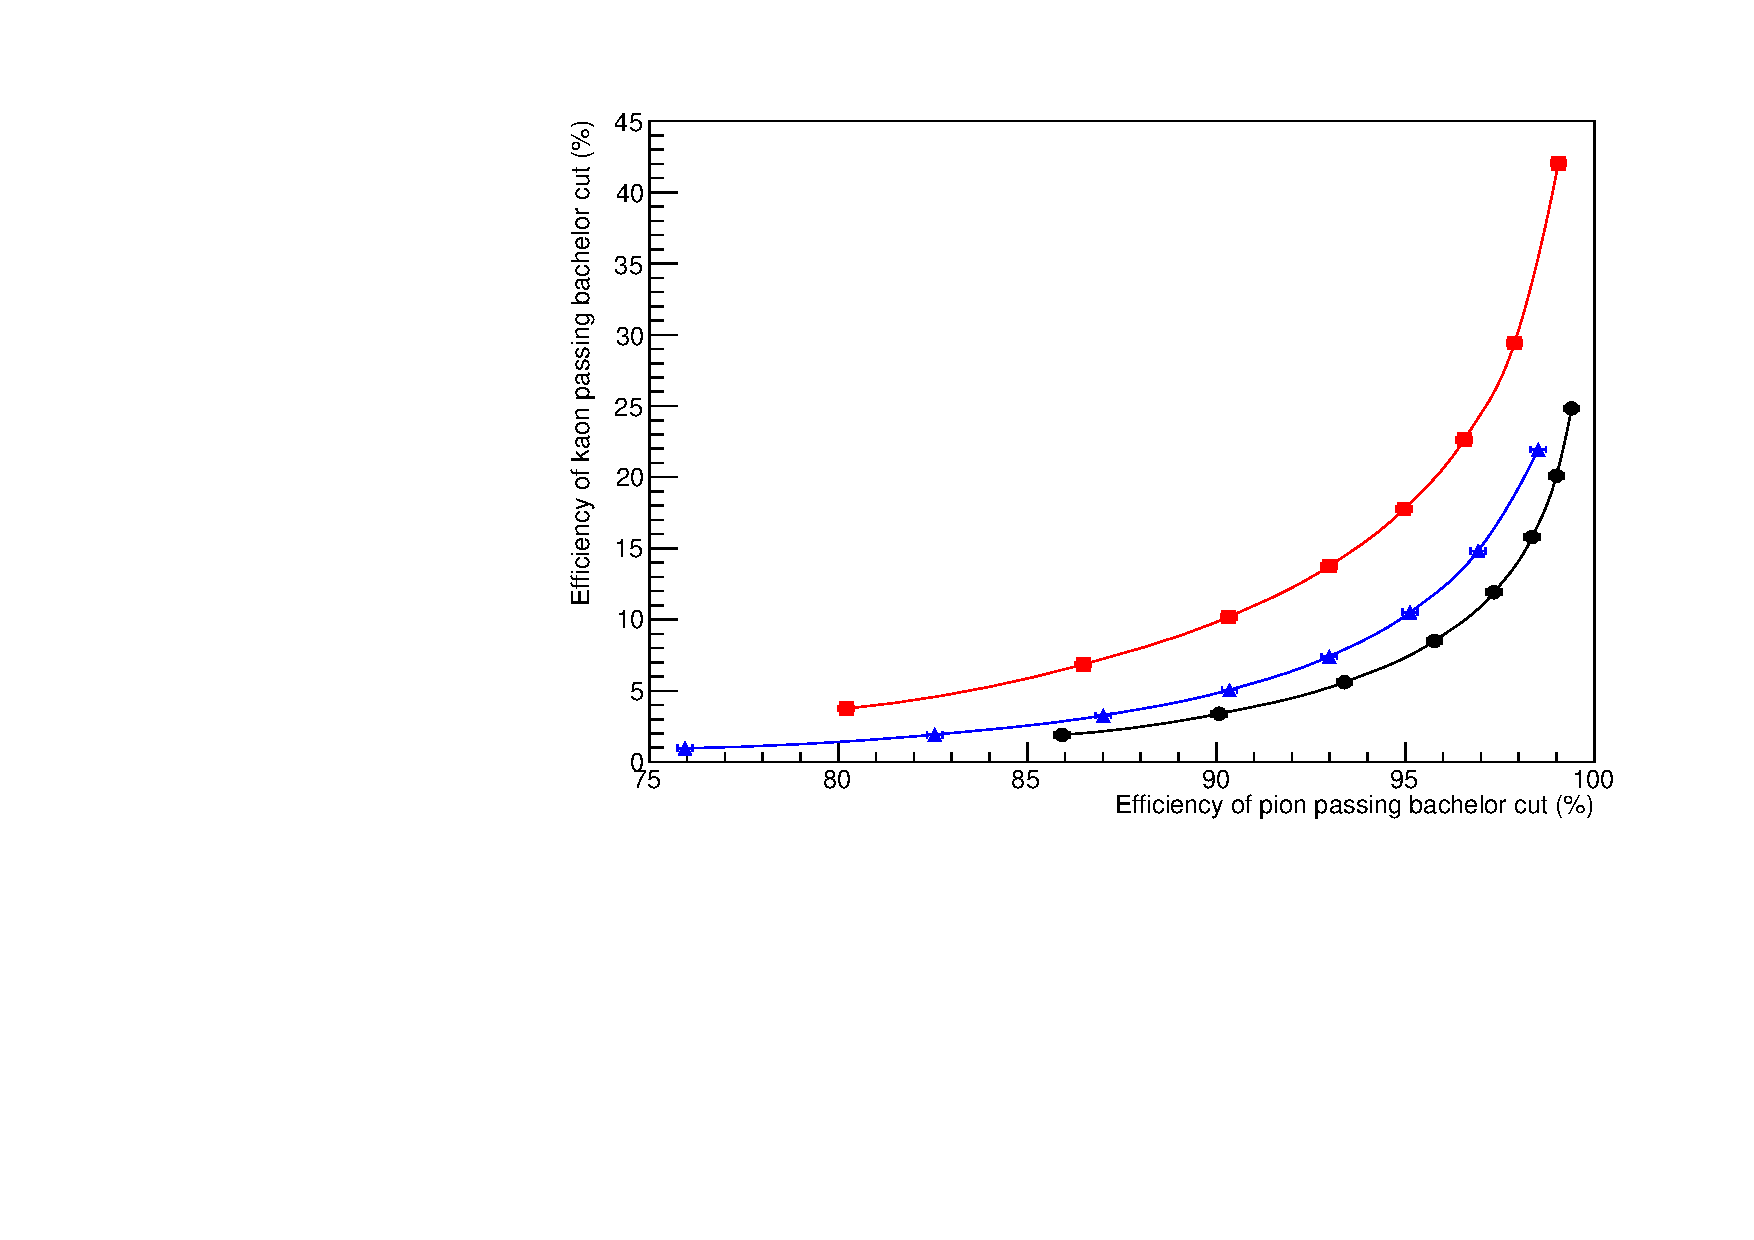
\includegraphics[width=0.5\linewidth]{figures/selection/pidOptimisation_bachelor.pdf}
\put(-150,100) {(a)}
\hfill
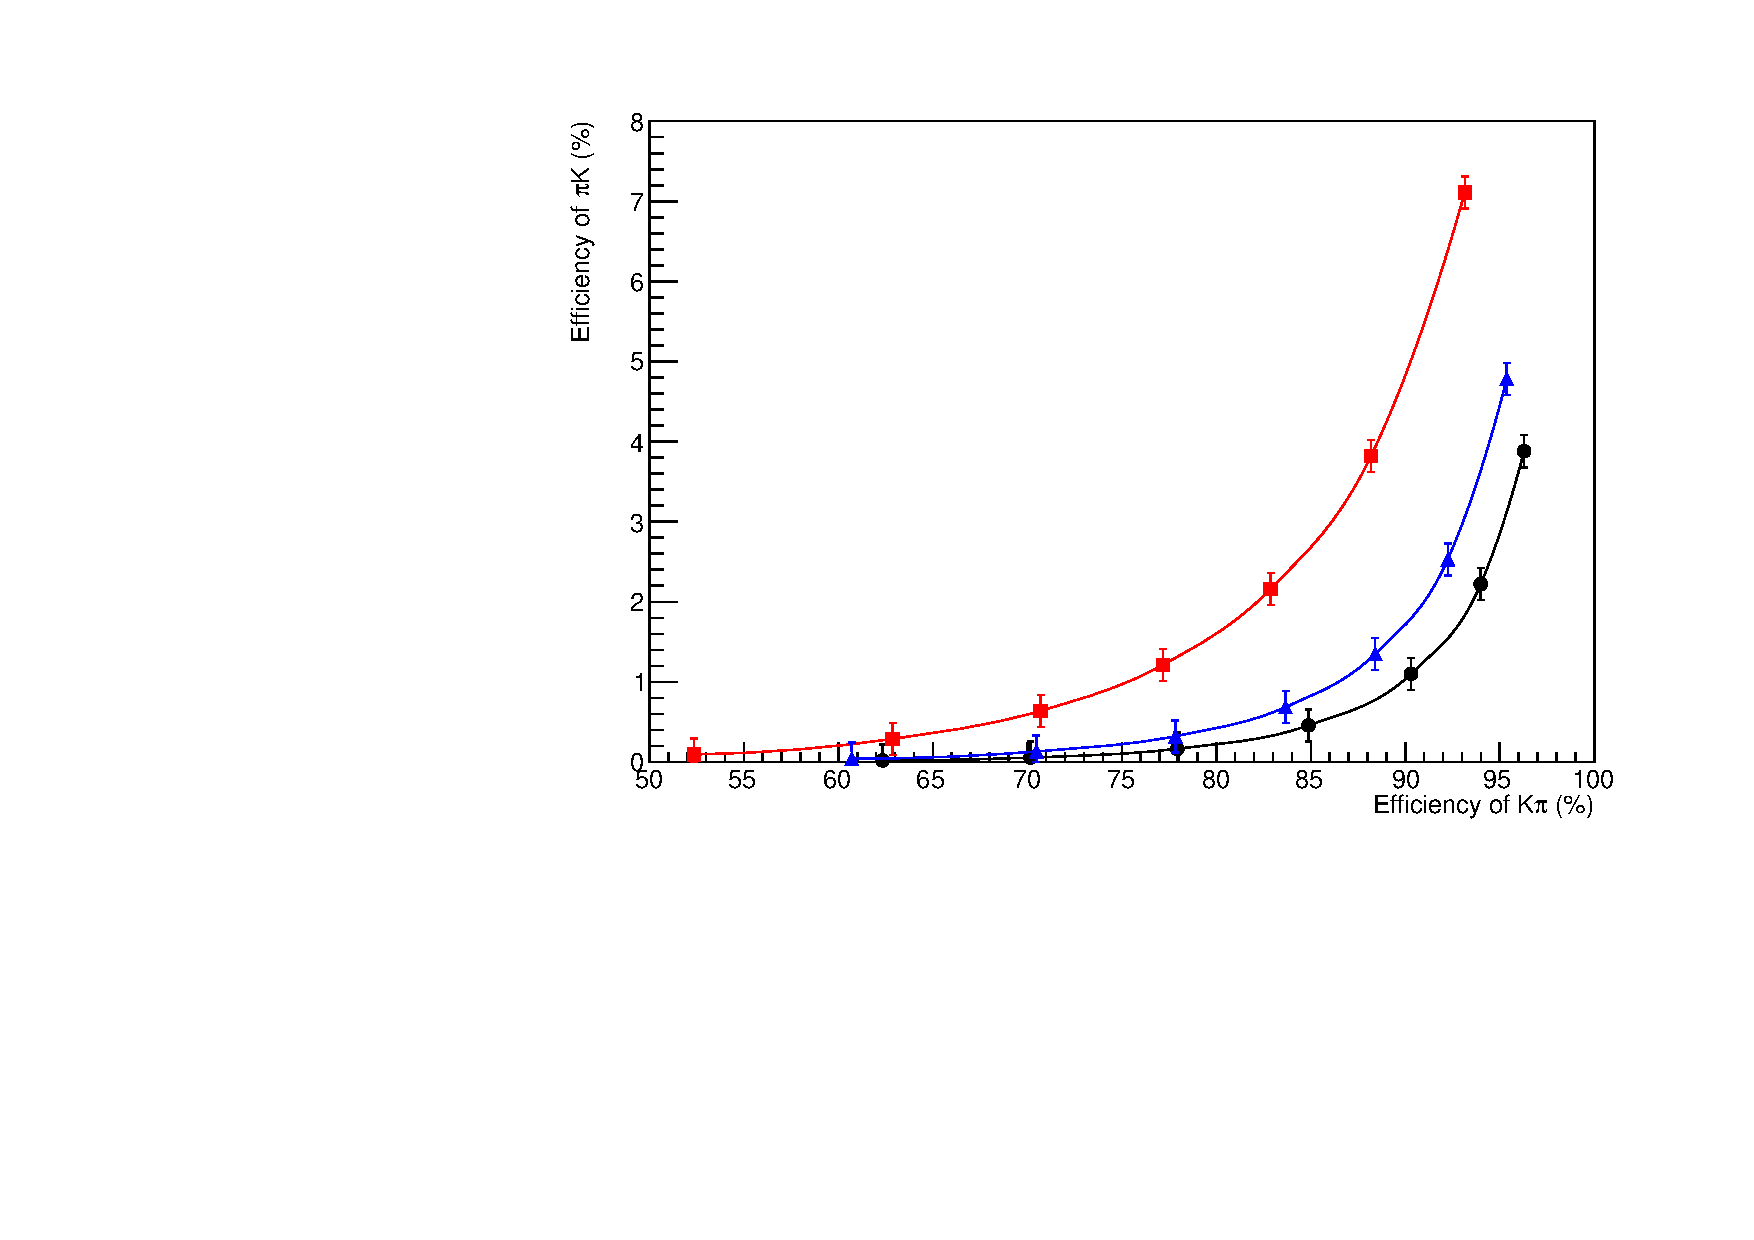
\includegraphics[width=0.5\linewidth]{figures/selection/pidOptimisation_Ddaughters.pdf}
\put(-150,100) {(b)}
\caption{PID efficiencies and misID efficiencies for various PID selections applied to (a) the bachelor pion, and (b) the D daughters. The black curve is for selections using $DLLK$, the red curve is for selections using $ProbNNpi$ and the blue curve is for selections using $ProbNNpi \times (1-ProbNNk)$}
\label{pidoptimisation}
\end{figure}

\subsection{Multiple candidates}
\label{sec:selection:multiplecandidates}

The selection may produce more than one signal event from the same B candidate. The rate of these multiple candidates was calculated after the final selection and only considering candidates in the range of the \CP fit (refitted \B mass $>$ 5230 \mev), see Section \ref{sec:massfit:range} for details on the fit range. The results are shown in Tables \ref{multiplecandidatesRun1} and \ref{multiplecandidatesRun2}. The rate is so low that no action is taken to remove the multiple candidates. In the ADS mode where it would have a significant effect, there are no multiple candidates.

\begin{table}[h]
\centering
\begin{tabular}{ccc}
\hline
& LL & DD \\
\hline
$K\pi$ & 0.005 (4) & 0.004 (9) \\
$K\pi$ & 0.008 (2) & 0.005 (3) \\
$KK$ & 0 (0) & 0 (0) \\
$\pi\pi$ & 0 (0) & 0 (0) \\
$\pi K$ & 0 (0) & 0 (0) \\
$K\pi\pi\pi$ & 0 (0) & 0.026 (7) \\
$\pi K\pi\pi$ & 0 (0) & 0.05 (1) \\
\hline
\end{tabular}
\caption{Multiple candidate rate for Run1. The number in brackets is the actual number of multiple candidates}
\label{multiplecandidatesRun1}
\end{table}

\begin{table}[h]
\centering
\begin{tabular}{ccc}
\hline
& LL & DD \\
\hline
$K\pi$ & 0.005 (7) & 0.005 (19) \\
$K\pi$ & 0.005 (2) & 0.004 (5) \\
$KK$ & 0 (0) & 0.006 (1) \\
$\pi\pi$ & 0 (0) & 0.011 (1) \\
$\pi K$ & 0 (0) & 0 (0) \\
$K\pi\pi\pi$ & 0 (0) & 0.012 (9) \\
$\pi K\pi\pi$ & 0 (0) & 0 (0) \\
\hline
\end{tabular}
\caption{Multiple candidate rate for Run 2. The number in brackets is the actual number of multiple candidates}
\label{multiplecandidatesRun2}
\end{table}

\clearpage
